%%%%%%%%%%%%%%%%%%%%%%%%%%%%%%%%%%%%%%%%%%%%%%%%%%%%%%%%%%%%%%%%%%%%%
% AGUJournalTemplate.tex

%% To submit your paper:
\documentclass[draft,linenumbers,onecolumn]{agujournal2019} % set options to [final] after final review
\usepackage{array}
\newcolumntype{P}[1]{>{\centering\arraybackslash}m{#1}}
\usepackage{url} %this package should fix any errors with URLs in refs.
\usepackage[inline]{trackchanges} %for better track changes. final option will compile document with changes incorporated.
\usepackage{soul}
\usepackage{multirow}
\usepackage{amsmath}
\usepackage{float}
\usepackage{placeins}
%%%%%%%
% As of 2018 we recommend use of the TrackChanges package to mark revisions.
% The trackchanges package adds five new LaTeX commands:
%
%  \note[editor]{The note}
%  \annote[editor]{Text to annotate}{The note}
%  \add[editor]{Text to add}
%  \remove[editor]{Text to remove}
%  \change[editor]{Text to remove}{Text to add}
%
% complete documentation is here: http://trackchanges.sourceforge.net/
%%%%%%%

% specific packages (added by Sebastian)
\usepackage{bm}
\usepackage{amssymb}

\journalname{Water Resources Research}

\begin{document}

\title{A Morphological Unit Approach to Optimizing 2D Hydrodynamic Model Calibration}

\graphicspath{ {./images/} }

%% ------------------------------------------------------------- %%
%
%  AUTHORS AND AFFILIATIONS
%
%% ------------------------------------------------------------- %%

\authors{Andres Heredia \affil{1},, Sebastian Schwindt\affil{1}, Silke Wieprecht\affil{1}, Sergey Oladyshkin\affil{2}}

\affiliation{1}{Institute for Modelling Hydraulic and Environmental Systems,
	Department of Hydraulic Engineering and Water Resources Management, University of Stuttgart, Stuttgart, Germany}

\affiliation{2}{Institute for Modelling Hydraulic and Environmental Systems, 
	Department of Stochastic Simulation and Safety Research for Hydrosystems, SC SimTech, University of Stuttgart, Stuttgart, Germany}


%% Corresponding Author:
% Corresponding author mailing address and e-mail address:
\correspondingauthor{Andres Heredia}{andres.heredia-hidalgo@iws.uni-stuttgart.de}

%% Keypoints, final entry on title page.
\begin{keypoints}
	\item Implementation of surrogate assisted calibration approach for 2D hydrodynamic models using Gaussian Process Regression and Bayesian Active Learning  
	\item Insert Key point
	\item Insert key point
\end{keypoints}

%% --------------------------------------------------------------- %%
%
%  ABSTRACT and PLAIN LANGUAGE SUMMARY
%
%% --------------------------------------------------------------- %%

%% \begin{abstract} starts the second page

% --- AUTHORS CLAP OUT THE COMMENT BAR --- --- --- --->>>

\begin{abstract}
% max. 250 words (curr. 249) -- A NEW WORD REQUIRES DELETION
	
	
\textit{KEYWORDS: Multitask Gaussian process regression, Bayesian calibration, Bayesian Active learning, Telemac2D, surrogate, morphological units}
\end{abstract}

\section*{Plain Language Summary}
% currently 196/200 words, accounting for AGU recommendations (https://www.agu.org/Share-and-Advocate/Share/Community/Plain-language-summary)

The real behaviour of rivers can be simulated using conceptual computer models. These models are often highly complex and computationally demanding because they must represent detailed, coupled physical processes such as water and sediment dynamics, requiring the introduction of several uncertain model parameters and hindering the identification of plausible parameter combinations which lead to acceptable resemblance to reality. To alleviate this, we use a machine learning-based model to approximate the behaviour of the complex model. With it, we perform data-driven stochastic analysis to identify parameter combinations that lead to a desired and plausible resemblance of the complex model to reality. We find that...   


\section{Introduction}

% State of art in modeling hydromorphological processes in presence of NbS and limitations
Anthropogenic activities in natural river corridors have significantly modified hydro-morphodynamic processes, resulting in permanent environmental changes and imposing unnecessary stress on species to adapt to these altered conditions \cite{grooten2018living, pasternack2020river}. The current need in the river engineeeing field is to explore viable alternatives to reverse these changes and establish stable, long-lasting solutions that restore environmental sustainability. Relevant studies in river restoration such as in \citeA{kail2007use,roni2015wood,grabowski2019current,neuhaus2021engineered} have explored the use of large woods (LW) as nature-based solutions, demonstrating positive outcomes in improving river ecosystem health with minimal potential impact. Similarly, studies developed by \citeA{follett2020momentum, schwindt2023fuzzylogic,schalko2024enhanced} have confirmed that large woods (LWs) create favorable heterogeneous velocity patterns in their wakes and contribute to aquatic life enhacement by interacting with the riverbed substrate. These studies highlight the importance of these hydrodynamic patterns to promote morphological variability and interconnected processes between surface water, sediment transport and river substrate matrix, which must be necessarily considered in restoration efforts.  Building on the findings of \citeA{schwindt2023fuzzylogic}, \citeA{scolari2025hydromorphodynamic} expanded the research in the field and developed a two-dimensional hydro-morphodynamic model that was able to identify potential zones of riverbed clogging in the presence of large wood (LW) structures. The latter opens up a new research direction where reliable numerical models can be a valuable asset in understanding coupled hydro-morphodynamic processes for river restoration. Indeed, a variety of numerical models and empirical approaches, each with its own advantages and limitations, have been developed to describe hydro-morphodynamic physical phenomena. However, they still struggle to accurately simulate the interplay between flow dynamics, morphological evolution, and sediment transport due to several hindrances \cite{nones2019numerical,kuhanestani2022hydraulic}. Hydro-morphodynamic models face significant challenges in improving reliability, such as spatial and temporal scaling, approximation schemes for solving fundamental PDEs (e.g., the Navier-Stokes equations for fluid dynamics or the Exner equation for sediment transport), high uncertainty in model parameters, computational demands, among others, making their implementation highly complex \cite{williams2016numerical,yassine2023numerical}.

% Hydro-morphodynamic model heterogeneity , different roughness zones, reserach gap
Despite their complexity, two-dimensional hydro-morphodynamic models have demonstrated being valuable tools for simulating coupled flow-sediment transport processes, offering a reasonable balance between accuracy and computational efficiency \cite{papanicolaou2008sediment}. In these models, hydrodynamic patterns play a key role in governing sediment motion which is, in fact, closely linked to bed roughness variability, as it reshapes the riverbed through processes of deposition and erosion \cite{lokin2023effect,mishra2020alluvial}. This roughness variability is usually simplified in numerical models by the assumption that the main channel material is homogeneous, which can be represented in modeling by establishing a constant roughness coefficient (i.e., Manning-Strickler coefficient) based on the general properties of the riverbed \cite{chow1959openchannel}. In contrast, studies such as \citeA{bunte2001samplinga,garcia2012complex} suggest that variations in flow patterns such as velocity and water depth along a river corridor in the form of run-riffle-pool sequences, can be effectively linked to spatial features of a river’s hydro-morphological structure. These spatial configurations are called morphological units (MUs) \cite{wadeson1994geomorphological,wyrick2014geospatial}; which are closely tied to sediment dynamics and spatial roughness variability across various spatial and temporal scales \cite{bunte2001samplinga}. Furthermore, this MUs roughness variability can be significantly influenced by dynamic events such as flush events or the presence of instream Nature-based Solutions (NbS) such as wood logs (LW), which introduce additional complexity in sediment transport and bed roughness dynamics.  This complexity, in fact, hinders any model´s predictive capacity. Thus, improving model reliability depends strongly on the implementation of optimized calibration and validation approaches that are able to consider multiple and sensitive parameters in hydro-morphodynamic models (i.e., roughness coefficients, hydrodynamic and sediment transport empirical coefficients, boundary conditions, etc) while considering their inherent uncertainties \cite{guerrero2012calibration,li2011twodimensional,bel2020calibration,scolari2025hydromorphodynamic}.

%multiparametric and time consuming---so we use surrogates? adding more data with two calibration targets?
Research studies such as in \citeA{villaret2016firstorder,beckers2018uncertainty,clare2022calibration} have applied advanced mathematical methods for sensitivity analysis of multiparametric hydro-morphodynamic models. Similarly, surrogate-assisted approaches have been used by  \cite{mohammadi2018bayesian,beckers2020bayesian} to quantify parameter uncertainties and support model comparison and calibration. The main goal of these analysis is to identify sensitive model paremeters, from which plausible combinations lead to the best fit between model outputs and measured data (i.e., calibration target) while reducing overall model uncertainty \cite{oberkampf2004verification}. A well- stablished approach to bypass difficulties in deterministic calibration approaches such as ill-posedness and model equifinality is treating the uncertainty of sensitive model calibration parameters as probability functions to perform stochastic analysis \cite{kim2016stepwise}. To accomplish this,Gaussian Process machine learning tools, aided by active learning techiques have been explored in recent studies for reservoir modeling applications \cite{schwindt2023bayesian, mouris2023stability} to approximate computationally demanding and multiparametric numerical models (i.e., high-complexity models) through surrogate models or metamodels trained with only a few samples or model runs from the complex model (e.i., input-output sets). These metamodels optimize the calibration and validation process by allowing the testing of a large number of parameter combinations within plausible ranges (i.e., competing models), and by incorporating data-driven approaches such as Bayesian Model Inversion \cite{mohammadi2018bayesian} to quantify parameter uncertainty. Surrogate-assisted calibration approaches have been tested in water engineering for single-output surrogates, meaning calibrating for a single calibration target. However, the physics in many natural processes are rarely single-output or isolated processes, rather better represented as multi-output processes \cite{ferreira2022multioutput} or inter-dependent tasks \cite{bonilla2007multitask}. These correlations between the outputs (i.e., water depth and velocity) can be captured by a multi-output surrogate model (i.e., Multitasks Gaussian Process as in \cite{bonilla2007multitask}) and leveraged for calibration purposes in hydro-morphodynamic river simulations. 

% 
To this end, the aim of this study is to perform Bayesian calibration and parameter uncertainty quantification of a 215-meter-long hydro-morphodynamic numerical model of a fish pass, where two large instream wood logs (LWs) were installed. The full complexity model incorporates a velocity–water depth-based delineation of morphological units (MUs) within the main channel, capturing spatial roughness variability across different scales. Furthermore, it simulates a gate-controlled flush event that accounts for sediment inflow, enabling the assessment of how variations in bed roughness influence water depths and flow velocities under sediment transport conditions.

A Gaussian Process (GP) metamodel approximates the full complexity model and is employed to perform stochastic analysis through Bayesian calibration of the five sensitive MU roughness coefficients depicting the riverbed variability and the critical Shields parameter for sediment transport. To make the stochastic calibration feasible, the study uses a multi-output Gaussian Process approach that simultaneously simulates two correlated output variables—water depth and velocity—which serve as calibration targets. Furthermore, the metamodel uses an active learning approach as proposed by \cite{oladyshkin2020bayesian3} to add additional training points based on relative entropy to improve the accuracy of the metamodel. 

Through this approach, the study aims to answer two research questions: First, how does a morphological unit delineation of the riverbed aid in increasing the effectiveness of model calibration? Second, how does the inclusion of two calibration quantities, such as water depth and velocity obtained from a multi-output Gaussian Process-based surrogate model, improve the uncertainty quantification of the considered calibration parameters during Bayesian calibration?

We hypothesize that a MU-based roughness delineation, combined with a sensitive sediment transport coefficient such as the critical Shields parameter, and the inclusion of more data (two calibration targets) in the Bayesian calibration process, narrows the probability distribution functions for highly uncertain parameters that are sensitive to the two calibration target quantities, and provides probabilistic regions where the uncertain parameter responses are more likely to fit measured data.  


\section{Materials and Methods} 
\label{Materials}
\cite{haag2001erosion}
\subsection{Fish pass at the Ering-Frauenstein power plant}
\label{subsec:Sec2.1 }
The present project develops in an artifitial, gravel-cobble riverbed fish pass located at the left bank of the Ering-Frauenstein water power plant. The fish pass was installed between 2018 and 2020 covering a length of approximately 2.6 km  and width between 5 m to 10 m measured at the base flow of  2~m$^3$/s. The channel overcomes a total height difference of approximately 10 m with a mean slope of 4.7\% forming meanders, pool-riffle sequences, gravel bars, and swales providing the necessary hydrodynamic and morphodynamic conditions to preserve endemic aquatic life in the Inn River \cite{schwindt2023fuzzylogic,zauner2020wie}. This study focuses on a 215-meter long stretch of the fish pass, between the abscissae 1450m and 1665m, with an average slope of 0.5\%. In January 2022, two large wood logs as Nature-based Solutions (NbS) for river restoration, hereafter referred to as 'LW', were installed perpendicular to the flow within the fish pass to assess their beneficial effects on riverbed declogging following an artificial flood of 9.7~m$^3$/s  \cite{schwindt2023fuzzylogic}. The two LW structures are located at local coordinates WGS 84 / UTM Zone 33N (363071.83, 5350214.56) for LWA and (363118.99, 5350254.67) for LWB. LWA works emerged and LWB works submerged at the base flow, but both work submerged during the peak flow event. Both structures generate backwater and wake effects with proven  hydrodynamic, morphodynamic and ecological benefitial effects \cite{schalko2021flow,schwindt2023fuzzylogic}.    
The Ering fish pass is a gate-regulated channel which fixes flow conditions enabling data extraction at multiple locations of interest with satisfactory outcomes. During artifitial flushing events, the channel receives discharges of up to 12 ~m$^3$/s, actively changing the grain size composition of the riverbed and its morphology depicted in highly detailed digital elevation models (DEMs) and visible present through high resolution orthopictures.


\begin{figure}[htbp]
	\centering
	\includegraphics[width=5.5in]{images/1_EringFishpass_domain.png}
	\caption{Study area  at the Ering fish pass (abscissae between 1450~m to 1665~m). Two wood logs, A (upstream) and B (downstream) are located at strategically points and where measured data have been taken. The project covers a meandering cobbel-gravel stretch of the fish pass transporting 2~$m^3$/s after a flush event of 9.7~$m^3$/s.   
	}
	\label{fig:StudyArea}
\end{figure}


\subsection{Bi-dimensional hydro-morphodynamic}
\label{sec:Sec2.2}

A 2D hydro-morphodynamic model of the Ering fish pass was created employing Telemac2D and Gaia. Telemac2D is a  highly versatile and applicable tool for two-dimensional hydrodynamic simulations used in a wide range of studies in free surface hydraulics. It uses a collection of computer program codes that iteratively solve the depth-averaged shallow water equations over an unstructured mesh through either finite element or finite volume methods and sets up the field for a sediment transport computation with Gaia \cite{galland1991telemac,hervouet2007hydrodynamics,tassi2023gaia}. Gaia, on the other hand, addresses sediment transport calculation and morphological evolution changes by considering spatial and temporal variability of sediment size classes and transport modes \cite{tassi2023gaia}. 

%The solved partial differential equations that are being iteratively solved are the following: 
%
%\begin{align}
%	&\frac{\partial h}{\partial t} + \vec{u} \cdot \nabla h + h \, \text{div} \, \vec{u} = 0, \tag{1} \\
%	&\frac{\partial u}{\partial t} + \vec{u} \cdot \nabla u + g \frac{\partial h}{\partial x} = D_x + S_x - g \frac{\partial Z_f}{\partial x}, \tag{2} \\
%	&\frac{\partial v}{\partial t} + \vec{u} \cdot \nabla v + g \frac{\partial h}{\partial y} = D_y + S_y - g \frac{\partial Z_f}{\partial y}. \tag{3}
%\end{align}
%
%where \( h \) represents the water depth, \( u \) and \( v \) denote the components of the velocity field, \( g \) is the acceleration due to gravity, \( D_x \) and \( D_y \) are the diffusion terms, \( S_x \) and \( S_y \) correspond to the source terms (including bottom friction, Coriolis force, wind stress, etc.), and \( Z_f \) indicates the bottom elevation.

%The diffusion terms are written as follows:

%\begin{align}
%	D_x &= \text{div}(v \, \nabla u) \tag{4} \\
%	D_y &= \text{div}(v \, \nabla v) \tag{5}
%\end{align} 

The current model utilizes a computational mesh that discretizes the simulation domain with triangular mesh elements with size averaging 0.55 m along the riverbed channel and 1 m for the floodplain mesh (see Fig.~\ref{fig:Mesh}).The detailed DEM, formerly in GeoTIFF format, possesses a resolution of 5 cm and is interpolated onto the computational mesh along with the roughness zones data. The model comprises a computational domain with a total of 11,738 nodes and 22,997 triangular elements and simulates an unsteady flow scenario, starting with a pre-flush base flow of 2~m$^3$/s, followed by a peak discharge of 9.7~m$^3$/s during 7 hour and returning to a post flush escenario with the same initial base flow. The upstream boundary condition was set as an unsteady inflow boundary , letting in liquid and solid mass fluxes according to the correponding hyrograph (see.... suplement material) and the downstream boundary condition as a water elevation - discharge relation defined by the Manning - Strickler criteria to assign the normal water depth for the corresponding discharge. 

For the hydrodynamic simulation, the model uses the Nikuratse friction law as expleined in \cite{hervouet2020telemac2d} and the effective roughness \(K_{s}\) as the flow resistence parameter describing the surface roughness height of the riverbed and banks \cite{nikuradse1933stroemungsgesetze,marriott2010hydraulic,webber2018fluid}. In studies such as \cite{meyer-peter1948formulas, ferguson2007flow, rickenmann2011evaluation} focusing to river applications, the Nikuradse roughness height is often referred to in terms of the characteristic riverbed particle diameters such as \(d_{50}\), \(d_{84}\), or \(d_{90}\) affected by a factor F as, for instance \( K_{s} = F \times d_{50} \) when using the mean particle size \cite{meyer-peter1948formulas,tassi2023gaia}. The effective roughness height is also associated with the Manning-Strickler roughness coefficient based on nomerous authors works.
The geometry mesh has in total 13 roughness zones, from which 5 correspond to a riverbeds subdivision based on morphological units (MU) and their corresponding Nikuradse coefficient \(K_{s}\) (see Fig.~\ref{fig:MU}). The additioal roighness zones are showed in the table.....  The subdivision's criteria based on the morphological units  and the corresponding values of \( K_{s} \approx F \times d_{50} \) will be thoroughly detailed in section \ref{sec:Sec2.5}.


Since \(d_{50}\) is usually a constant value taken from laboratory tests, the initial model considers the criterion of F = 3. The values of \(K_{s}\) used as roughness coefficients in the model are refined by the facot F which are taken from uniform distribution functions with fixed limits which led from meaningful roughness coefficient values for gravel-cobble rivers. Table~\ref{tab:model_characteristics} shows a summary of the assigned characteristics of the numerical model.


% (I CAN USE THIS LATER IN THE DOCUMENT)According to \cite{meyer-peterFormulasBedLoadTransport1948} the Nikuradse roughness height  The roughness height is of the river from measured data \(d_{90}\)
%% In fact, it is not possible to generalize the value of 3.26 for all alluvial rivers, for this reason the experiment employed the Nikuratse roughness as \(F\) * \(d_{50}\), in which \(F\) constitue an uncertain factor that affects the mean roughness height of the riverbed. 


\begin{figure}[!htbp]
	\centering
	\includegraphics[width=5.5in]{images/2_EringFishpass_mesh.png}
	\caption{Mesh properties of the Ering fish pass model.}
	\label{fig:Mesh}
\end{figure}


\begin{table}[H] 
	\centering
	\caption{Model Characteristics.}
	\begin{tabular}{p{4cm} p{10cm}}
		\hline
		\multicolumn{1}{c}{\textbf{Model Specifications}} & \multicolumn{1}{c}{\textbf{Description}} \\ \hline
		\multirow{2}{4cm}{Boundary Conditions} & \textbf{Upstream}: Prescribed discharge of 2~m\textsuperscript{3}/s (e.g., base flow conditions). \\ 
		& \textbf{Downstream}: State-discharge relation between discharge and normal water depths. \\ \hline
		\multirow{2}{4cm}{Mesh Size} & \textbf{Main channel}: 0.55 m. \\ 
		& \textbf{Floodplains}: 1 m. \\ \hline
		Roughness Coefficient & Nikuradse roughness height \(d_{90}\). \\ \hline
		MU Subdivision & Glide, Riffles, Run, Pool, Slackwater. \\ \hline
		Nikuradse Roughness & \( K_{\text{pool}} \sim U(0.011, 0.79) \), 
		\( K_{\text{slackwater}} \sim U(0.011, 0.79) \), 
		\( K_{\text{glide}} \sim U(0.0016, 0.056) \), 
		\( K_{\text{riffle}} \sim U(0.0016, 0.056) \), 
		\( K_{\text{run}} \sim U(0.056, 0.79) \). \\ \hline
	\end{tabular}
	\label{tab:model_characteristics}
\end{table}
 \vspace{-20pt}      
\FloatBarrier
\subsection{Hydrodynamic Delft3D-FLOW Model}
\label{sec:Delft3D}

% Model intro
A 3d hydrodynamic numerical model of the SR was set up with the Delft3D-FLOW software. The software solves the Reynolds-averaged Navier Stokes equations and the continuity equation for incompressible fluids with the Boussinesq approximation for buoyancy-driven convection \cite{deltares_simulation_2022}. In the here used Delft3D-FLOW model, we took advantage of the software's computational efficiency with its z-layer model for 3d discretization in space based on a finite difference scheme \cite<e.g.,>{platzek_accurate_2014}. The discretization in time uses the alternating direction implicit method \cite<in line with>{morgan_use_2020}. In contrast to CFD software (e.g., OpenFOAM) using hexahedral meshes for the representation of complex 3d structures, the vertical dimension of a 3d mesh in Delft3D-FLOW is based on multiple layers of a two-dimensional (2d) mesh.

% Bussinesq approximation
The Boussinesq approximation simplifies the simulation of heat transfer in fluids (here: water) in which the temperature varies in space. The approach ignores changes in the fluid properties except for the fluid density, which only occurs as a multiplier of the gravitational acceleration. Moreover, the Boussinesq coefficient quantifies the momentum effect of the non-uniform velocity distribution over the water depth. Since the Boussinesq term appears in the advective acceleration in the shallow water equations, it can also be treated as a purely numerical calibration parameter to adjust the amount of fluid inertia to be considered in a simulation \cite{kundu_fluid_2008, yang_boussinesq_2018}. The Boussinesq approximation (or hypothesis) is referred to as the (Boussinesq) eddy viscosity assumption in the following and according to the Delft3D-FLOW nomenclature.

% k-epsilon model and eddy viscosites
With the eddy viscosity (Boussinesq) hypothesis, a $k-\epsilon$ turbulence closure was defined along with horizontal and vertical eddy viscosities. The eddy viscosities are proportionality factors for the turbulent energy transfer resulting from moving eddies and leading to tangential stresses \cite{blazek_chpt7_2005}, which we considered drivers for the observed flow velocity and water temperature patterns. 

% model for eddy viscosities
The horizontal eddy viscosity~$\nu_{h}$ varied in this study as a function of the vertical eddy viscosity~$\nu_{v}$, and the background horizontal eddy viscosity~$\nu_{h}^{back}$ \cite{deltares_simulation_2022}:

\begin{equation}
	\label{eq:nuh}
	\nu_{h} = \nu_{v} + \nu_{h}^{back}
\end{equation}

$\nu_{v}$~affects the 3d turbulence and Delft3D-FLOW calculates $\nu_{v}$ based on the $k-\epsilon$ turbulence closure (see also the supplemental material).

% showing extra luv for nu_h_back as calib param
The background horizontal eddy viscosity $\nu_{h}^{back}$ was one of the calibration parameters in this study (see summary in the next section). It represents 2d turbulence and accounts for multiple hydrodynamic phenomena. In a stratified reservoir, turbulent eddy viscosity at stratification interfaces drops to zero and vertical mixing reduces to molecular diffusion. However, zero eddy viscosity is not physically correct because of the presence of internal waves, which are continuously generated by different sources and turbulence (i.e., vertical mixing) \cite{hodges_modeling_2000}. Since internal waves are not explicitly considered in the Delft3D-FLOW turbulence model, they were added spatiotemporally using the background eddy viscosity~$\nu_{h}^{back}$ \cite{deltares_simulation_2022}.

% also need a diffusion parameter
While adjusting the eddy viscosity allowed us to mimic the mixing due to momentum, we additionally considered diffusivity that aids in representing the mixing of heat. Analogously to how Delft3D-FLOW calculates viscosities, the horizontal eddy diffusivity~$\Delta_{h}$ is a function of the constant vertical eddy diffusivity of~$\Delta_{v}$~=~10$^{-6}$~m$^{2}$~s$^{-1}$, and the background horizontal eddy diffusivity~$\Delta_{h}^{back}$ \cite{deltares_simulation_2022}:

\begin{equation}
	\label{eq:Duh}
	\Delta_{h} = \Delta_{v} + \Delta_{h}^{back}
\end{equation}

In addition to $\nu_{h}^{back}$, the background horizontal eddy diffusivity~$\Delta_{h}^{back}$ was also a calibration parameter in this study (see also next section). The sub-grid scale horizontal eddy viscosity and diffusivity were zero in our model.

% domain geometry and discretization
Regarding spatial abstraction, a boundary-fitted domain discretized the reservoir bathymetry (\figurename{~\ref{fig:sr_map}}) into 27 vertical layers with 5,299 tetrahedral cells each. In consequence, the average cell size was 9x15x1.7~m in the $x$, $y$, and $z$ directions, respectively. We also tested the model with more (up to 40) and fewer (minimum 9) layers, which either led to unacceptably long computing time or could not represent variations in the vertical velocity profiles during pump operation. For the latter reason, we also used the z-layer (not $\sigma$-layer) model for vertical discretization.

% boundary conditions
The unsteady liquid boundaries were defined with the water level and the discharge time series provided for the three affluents and at the intake tower, corresponding to a one-week-long simulation (August~1 at 00:00~AM through August~7 at 00:00~AM, 2016). Figure~\ref{fig:liquid-bound-fluxes} shows the prescribed liquid boundary characteristics. The bottom roughness was set to \textit{Manning} with an equivalent global value of 0.015, which was not modified in the calibration process. Other physical processes affecting the flow pattern were considered in the form of air temperature and wind (processes module and the above-introduced meteorological data) because those are known to affect flow velocities in the upper layers of reservoirs, and therefore, density stratification \cite{zhen-gang_hydrodynamics_2008, dissanayake_delft3d_2019}.

% initial conditions
The initial conditions corresponded to a water level of 661.34~m and a constant (in $x, y, z$) water temperature profile with possible values defined within a range between 5$^{\circ}$C and 30$^{\circ}$C. The water temperature profile was implemented in Delft3D-FLOW at the mesh boundary of the intake tower along with the discharge (i.e., liquid) boundary.

\begin{figure}
	\centering
	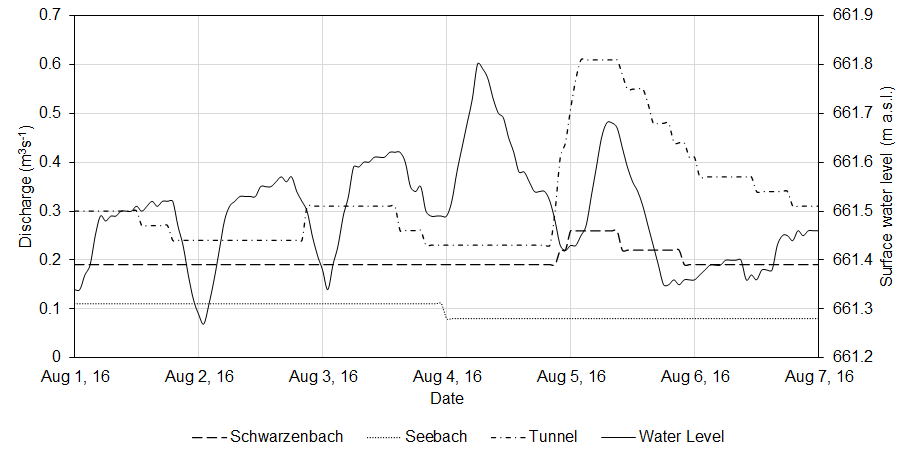
\includegraphics[width=14.5cm]{inflow-series.png}
	\caption{Flow series and water levels defined at the liquid boundaries of the numerical model.}
	\label{fig:liquid-bound-fluxes}
\end{figure}

A run of the Delft3D-FLOW model took an average of 12.8 hours on a 6-core computer with 2.3~GHz per core and 16~GB memory. The simulations ran on all 6 cores. The output was written hourly. The supplementary material contains more details about the numerical model.

\subsection{Relevant Calibration Parameters}
\label{sec:CalibParams}

% how we chose them
The identification of relevant calibration parameters is the baseline for any model calibration. We identified three relevant calibration parameters based on other studies \cite<e.g.,>{ahlfeld_case_2003, chanudet_3d_2012, dissanayake_delft3d_2019, goudsmit_application_2002}, our experience, and preliminary tests with the Delft3D-FLOW model of the SR.

% name the three
The three selected calibration parameters are listed in \tablename{~\ref{TableParam}} and embraced background horizontal eddy viscosity $\nu_{h}^{back}$, background horizontal eddy diffusivity $\Delta_{h}^{back}$, and the initial water temperature at the intake tower~$T_{tow}$ (i.e., the liquid boundary of the computational mesh). We combined the values~$\omega$ of the three calibration parameters into a single vector~$\Omega$ that was required for the below-described Bayesian calibration:

\begin{equation}
	\Omega = \{\omega_{\nu_{h}^{back}}, \omega_{\Delta_{h}^{back}}, \omega_{T_{tow}}\}
	\label{eq:parameterVector}
\end{equation}

% why these?
We chose the horizontal eddy viscosity and diffusivity because they have a strong influence on the turbulent viscosity terms of the advection-diffusion equations for heat transport (Boussinesq approximation). In addition, both parameters result from the simplification hypotheses of the mathematical equations, and hence, are typical candidates for calibration.

% why water temperature?
We chose the initial water temperature at the intake tower ($\omega_{T_{tow}}$) as a calibration parameter because it has a considerable effect on the currents in the SR. Due to pump and turbine operations, thermal stratification, and missing monitoring data of water temperature directly at the intake tower (only available at the measurement station, cf. the star in \figurename{~\ref{fig:sr_map}}), the water temperature introduced considerable model uncertainty and it could reportedly not be well reproduced in other studies \cite<e.g.>{dissanayake_delft3d_2019}. The initial water temperature profile was key to the physically unreasonable scenario explained in the test procedure section below.

% value ranges
\tablename{~\ref{TableParam}} shows the considered value ranges (interpreted as uniform probability distributions) for the three calibration parameters, which stem from the literature \cite<see supplemental material and>{dong_lake_2020, bermudez_res_2018, li_efdc_2010, kosucu_delft3d_2019, dissanayake_delft3d_2019, salehi_delft3d_2017}, the Delft3D user manual \cite{deltares_simulation_2022}, and our experience. These distributions formed the prior distributions to be updated to posterior distributions in the Bayesian calibration (see next section).

\begin{table}[h]
	\centering
	\caption{Calibration parameters and their value ranges~$(\mbox{min}, \mbox{max})$ for uniform distributions $\mathcal{U}(\mbox{min}, \mbox{max})$ considered in this study.}
	\begin{tabular}{l c c c} 
		\hline
		%\multicolumn{3}{l}{Calibration Parameters} & Prior distribution \\
		Parameter name & Symbol & Units & $\mathcal{U}(\mbox{min}, \mbox{max})$  \\
		\hline
		Background horizontal eddy viscosity &  \(\nu_{h}^{back}\) & m$^2$s$^{-1}$ & $\mathcal{U}(0.1, 5)$  \\
		Background horizontal eddy diffusivity& \(\Delta_{h}^{back}\) & m$^2$s$^{-1}$ & $\mathcal{U}(0.1, 5)$ \\
		Initial water temperature (intake tower) & \(T_{tow}\) & \(^\circ\)C & $\mathcal{U}(5, 30)$ \\
		\hline
	\end{tabular}
	\label{TableParam}
\end{table}


\subsection{Bayesian Calibration Accelerated by Emulators and Active Learning}
\label{sec:bayesCal}

% The general Bayes:
A Bayesian calibration is a specific form of Bayesian updating through Bayes' theorem:

\begin{equation}
	p\left( \mathbf{\Omega} \vert \mathbf{D},\mathcal{M} \right) = \frac{p\left( \mathbf{D} \vert \mathbf{\Omega},\mathcal{M} \right) \cdot p\left( \mathbf{\Omega}\vert \mathcal{M}\right) }{p\left( \mathbf{D}\vert\mathcal{M}\right) }
	\label{eq:Bayes}
\end{equation}

where $p(\cdot)$ denotes probability density functions (pdfs). $\mathbf{\Omega}$~denotes the collection (vector) of calibration parameters for the deterministic model $\mathcal{M}$ according to Equation~\ref{eq:parameterVector}, and $p(\mathbf{\Omega} | \mathcal{M})$ denotes the prior pdf of the parameters in that model. It contains expert knowledge about the parameters, which is already available before the calibration. $\mathbf{D}$~denotes the collection (vector) of calibration data. $p(\mathbf{D} | \mathbf{\Omega} , \mathcal{M})$~is called \textit{likelihood}. It expresses (as a function of the parameter values $\mathbf{\Omega}$) how statistically likely it is to observe the data $\mathbf{D}$ if the combination of $\mathbf{\Omega},\mathcal{M}$ was true. The combination of prior information and calibration data updates the prior distribution $p(\mathbf{\Omega}|\mathcal{M})$ to the posterior distribution $p(\mathbf{\Omega} \vert \mathbf{D},\mathcal{M})$. By definition, the posterior distribution is more informative than (or at least as informative as) the prior distribution \cite{box_bayesian_1973, oladyshkin_connection_2019}. The denominator $p(\mathbf{D}|\mathcal{M})$, often referred to as Bayesian model evidence (BME, see below), plays an important role in (competing) model selection problems. The BME is merely a normalizing constant in this equation but can assist in error diagnosis.

% specification to our context
In this study, the model $\mathcal{M}$ was the full-complexity Delft3D-FLOW model (see above), calibration parameters were the background horizontal eddy viscosity and diffusivity as well as the initial water temperature (see Table \ref{TableParam}), and measurement data~$\mathbf{D}$ consisted of flow velocity and/or water temperature recordings (see above).

% Likelihood definition
What remained to be defined is the functional form of the likelihood~$p(\mathbf{D} \vert \mathbf{\Omega}, \mathcal{M})$ in Equation~\ref{eq:Bayes}. A typical assumption is that there is a measurement error~$\boldsymbol{\varepsilon}$ (i.e., residuals) between the model and observable reality, which can be derived from the following expression:

\begin{equation}
	\mathbf{D} = \mathcal{M}(\mathbf{\Omega}) + \boldsymbol{\varepsilon}
	\label{eq:residuals}
\end{equation}

The errors (stacked as a vector) typically have zero mean (no systematic errors) and a variance~$\sigma^2_{\varepsilon,D}$ that resembles the imprecision of measurements. The most common distributional assumption for measurement errors is Gaussian, and errors for different data items are uncorrelated. We followed this common assumption and obtained:

\begin{equation}
	p(\mathbf{D} \vert \mathbf{\Omega},\mathcal{M}) = 
	2\pi^{-\frac{n}{2}}\vert \mathbf{R} \vert^{-\frac{1}{2}}
	\exp\bigg[
	-\frac{1}{2}\big( \boldsymbol{\varepsilon}^T \mathbf{R}^{-1} \boldsymbol{\varepsilon}
	\big)\bigg]
	\label{eq:like}
\end{equation}

where $n$ is the number of data items (i.e., the number of measurements in $\mathbf{D}$ and of corresponding residuals in $\boldsymbol{\varepsilon}$) and $\mathbf{R}$ is the (co-)variance matrix of measurement errors (sized $n\times n$). In our case, $\mathbf{R}$ was a diagonal matrix populated by the variances $\sigma^2_{\varepsilon,D}$ per data item. The error variance (imprecision) of the measurement data in this study had a standard deviation of 2$^{\circ}$C for water temperature and 3~mm~s$^{-1}$ for flow velocity measurements.

% from prior to posterior in theory
Based on the posterior distributions, we extracted so-called maximum likelihoods of the calibration parameters (i.e., the location of an optimum in the likelihood function), which led to the best possible agreement with the measurement data \cite{beckers_bayesian_2020}. Likewise, maximum-a-posteriori calibration parameter values can be extracted (i.e., the optimum of the joint posterior distribution), which correspond to the best possible compromise between priors and data. For uniform distributions as used in this study, both sets of parameter values coincide and the posterior distribution characteristics represent the post-calibration uncertainty of the parameters.

% how to solve... need surrogate
Typical assumption-free computational methods to evaluate the Bayesian theorem in Equation~\ref{eq:Bayes} are computationally inefficient Monte-Carlo or Markov-Chain Monte-Carlo methods \cite<e.g.,>{smith_bayesian_1992}. These methods are particularly inefficient when a model~$\mathcal{M}$ is computationally expensive (e.g., if a Delft3D-FLOW run takes 12.8 hours on average), because these methods will make the model easily run millions of times to yield a good approximation of Equation~\ref{eq:Bayes}. To bypass long computing times, a surrogate model response~$\mathcal{S}(\mathbf{\Omega})$ was used to replace~$\mathcal{M}$ in the computation of residuals (Equation~\ref{eq:residuals}) with a much faster approximation:

\begin{equation}
	\mathcal{S}(\mathbf{\Omega}) \approx \mathcal{M}(\mathbf{\Omega})
	\label{eq:surrogate}
\end{equation}

% final Approximation of Bayes Cal with Surri
With a suitable surrogate model, speed is no longer an issue because it runs easily a million times faster than a full-complexity model \cite{beckers_bayesian_2020}. That is, a surrogate model enabled us to run 10\textsuperscript{6} random Monte Carlo realizations drawn from the prior pdfs of the calibration parameters. Then, we evaluated the surrogate model response~$\mathcal{S}$ for every realization, computed the (approximate) residuals with Equation~\ref{eq:residuals}, calculated each realization's likelihood with Equation~\ref{eq:like}, and used rejection sampling \cite{smith_bayesian_1992} to approximate the posterior distribution in Bayes' theorem (i.e., the left side of Equation~\ref{eq:Bayes}).

% Surrogate quality and construction and active learning
The approximation quality of the surrogate model had to be appropriate for the calibration task. The surrogate model's quality strongly depends on its construction method, including the selection of so-called training runs with the initial full-complexity model \cite{busby_hierarchical_2009}. This is where active learning becomes relevant: the training runs should concentrate mostly on high-likelihood areas, which are not known \textit{a priori}. This is the starting point for an iterative process called active learning that incrementally improves the surrogate model in currently found high-likelihood regions, and subsequently refines the identification of high-likelihood regions.

% We use GPE in BAL
Here, we used a Gaussian process emulator (GPE) as a surrogate model and Bayesian active learning (BAL) for efficient training. The theoretical background for GPEs and the used BAL technique can be found, for example, in \citeA{rasmussen200gpe} and \citeA{oladyshkin_bayesian3_2020}. To set up the GPE in this study, we applied a squared exponential kernel. This kernel required specifications of length scales and variance as hyperparameters, and we used the \texttt{fitrgp} function in \citeA{matlab_fit_2018} to choose their values. For iterating between training and Bayesian updating, we implemented the iterative BAL technique described in \citeA{oladyshkin_bayesian3_2020}. The BAL builds on a combination of preliminary Bayesian updating and information theory \cite{oladyshkin_connection_2019} to identify the next-best parameter set for training. Here, we used it to find the best out of 1,000 randomly proposed next-value candidates in every iteration. After every new training run, we re-iterated the hyperparameters and re-trained the GPE.

% convergence criteria
The BAL technique needs stopping criteria to identify that the iterations converge toward a final quality level. For this purpose, we tracked Bayesian model evidence (BME, see denominator in Equation~\ref{eq:Bayes}) and the so-called relative entropy in the BAL iterations. Here, we approximated the full-complexity model BME$_{\mathcal{M}}$ based on the GPE-surrogate model~BME$_{\mathcal{S}}$:

\begin{equation}
	\textbf{BME}_{\mathcal{M}} \equiv p_{\Omega}(\textbf{D} \vert {\mathcal{M}}) \approx \textbf{BME}_{\mathcal{S}} \equiv p_{\Omega}(\textbf{D} \vert {\mathcal{S}}) .
	\label{eq:bal_bme}
\end{equation}

The BME expresses as an integral quantity the average goodness of fit of the model, relative to the prior distribution. If the surrogate model response~$\mathcal{S}$ converges toward the full-complexity model response~$\mathcal{M}$ during the BAL, then BME$_{\mathcal{S}}$ converges toward BME$_{\mathcal{M}}$ and stabilizes. In addition, relative entropy, also known as Kullback-Leibler divergence $D_{KL}$, quantifies the information gain from the prior to the posterior distributions of the calibration parameters, and it was approximated with:

\begin{equation}
	\label{eq:re}
	D_{KL} [p(\Omega \vert \textbf{D},\mathcal{M}), p(\Omega \vert \mathcal{M})] \approx D_{KL} [p(\Omega \vert \textbf{D},\mathcal{S}), p(\Omega \vert \mathcal{S})] .
\end{equation}

Also $D_{KL}$ stabilizes when the surrogate model response converges toward the full-complexity model response. Thus, we continued the BAL iterations until both the BME and $D_{KL}$ converged toward a constant. In addition, BME and $D_{KL}$ were criteria for selecting training points in the BAL iterations. For details on the here-used approximation methods, in particular, regarding the GPE-surrogate model and BAL, see \citeA{oladyshkin_bayesian3_2020}.


\subsection{Test Procedure}
\label{sec:test-proc}

% global procedure
Initially, we ran the full-complexity, hydrodynamic, numerical 3d model (Delft3D-FLOW) of the SR 30 times to constitute the baseline for the BAL iterations. Next, we calibrated the three calibration parameters in the GPE-surrogate-assisted BAL iterations (see above). The prior calibration parameter distributions are listed in \tablename{~\ref{TableParam}}.
We used the available calibration data in the form of depth-averaged horizontal flow velocity and water temperature profiles at the measurement station (see \figurename{~\ref{fig:sr_map}}) in the three below-described scenarios. We considered the calibration complete when additional training points in the BAL iterations did not yield an improvement in BME (Equation~\ref{eq:bal_bme}) and relative entropy (Equation~\ref{eq:re}). To verify convergence, we logged the BME and relative entropy at the end of every iteration. Finally, we implemented the maximum likelihoods resulting from the posterior distributions of the last BAL iteration to re-run the full-complexity and GPE-surrogate models at the end of each below-defined scenario. In particular, we defined three scenarios to test the two hypotheses we formulated at the end of the introduction: 

(i)~A reservoir model with a physically inappropriate calibration setting can appear to correctly reproduce measurement data.

(ii)~The shape of posterior distributions points to physically unreasonable calibration results.

% scenarios
To test the hypotheses, three calibration scenarios with varying physical correctness were defined. These three scenarios were one all-data scenario (0), and two single-data set scenarios (1 and~2), in which we applied the flow velocity and water temperature measurement data separately from each other for Bayesian calibration.

% scenario 0
The all-data scenario~0 used both the flow velocity and water temperature measurement data from the measurement station to optimize the three calibration parameters. Computationally, this scenario was the most expensive because the number of training runs for the surrogate model scaled exponentially with the number of calibration parameters.

% scenario 1
Scenario~1 only used the flow velocity data to calibrate all three parameters, although the data were primarily useful to calibrate the horizontal eddy viscosity and diffusivity. This scenario was aimed at a physically more correct calibration toward heat-independent, short-term flow velocity patterns driven by pump and turbine operations. Thus, scenario~1 was physically better conditioned than the other scenarios because it only calibrated toward data that can be reasonably well reproduced by the Delft3D-FLOW model.

% scenario 2
Scenario~2 only used the water temperature data to calibrate all three parameters. Thus, the Bayesian calibration process had to attempt stratifying the reservoir (i.e., to match the measured water temperature profiles) based on an initially constant (over depth) water temperature profile at a distance of 270~m (i.e., at the intake tower).

% link scenarios to hypotheses
According to the above-mentioned literature \cite<e.g.,>{zhang_thermal_2020}, stratification within a simulation time of 6 days (real-time) is physically unlikely, which means that scenarios~0 and~2 corresponded to (partially) non-reasonable calibration frameworks because of too short simulation times. If the Bayesian calibration still succeeded (in terms of statistical scores) in calibrating the model seemingly well, we assumed that the model was poorly conditioned and evidence to support hypothesis~(i) was provided.

In contrast to lump-sum statistics (e.g., the \textit{RMSE}), we expected Bayesian calibration to indicate uncertainty related to the calibration results, which would not be visible after subjective trial-and-error calibration. Thus, if the physically more unreasonable scenarios~0 and~2 led to more uncertain posterior distributions and wrong bulk mixing parameters than the better-constrained scenario~1, evidence supporting hypothesis~(ii) was provided. In particular, we attempted to verify that high uncertainties in posterior distributions were consistent with the physical soundness of the calibration frameworks of the scenarios.

\tablename{~\ref{tab:scenarios}} summarizes the three test scenarios along with the number of BAL iterations, observations, and measurement data used per scenario. The number of BAL iterations anticipates the results and was driven by reaching the convergences of BME and relative entropy (see details in the results section). Note that we were using the depth-averaged horizontal flow velocity~$U$ for the Bayesian calibration, which was necessary to compare the results of the depth-averaged output of Delft3D-FLOW with the measurement data. In particular, the Bayesian framework \cite{oladyshkin_bayesian3_2020} can currently only work with one measurement point per x-y coordinate. It cannot deal with vertically varying velocities because of the resulting dimensionality of calibration vectors. For instance, if Bayesian calibration was extended to the third dimension in space, the response surface would have an additional dimension. Because the total of posterior probabilities still needed to sum up to 1, the additional dimension would decrease the prior output space to infinitesimally small numbers, which would all be rejected in the rejection sampling step \cite{smith_bayesian_1992,oladyshkin_bayesian3_2020}. The problem of too small (too close to zero) probabilities in the framework of active learning is also referred to as \textit{curse of dimensionality} \cite{bellman_dynamic_1957}, which is discussed in detail by \citeA{mouris_stability_2023}.

\begin{table}
	\caption{The three scenarios defining the frameworks for the Bayesian calibration as a function of involved measurements of depth-averaged horizontal flow velocity~$U$ and water temperature~$T$ at the measurement station.}
	\label{tab:scenarios}
	\centering
	\begin{tabular}{P{2cm} P{4cm} P{3cm} P{2cm}} 
		\hline
		Data scenario & \# of BAL iterations & Measurement quantities involved & \# of observations \\
		\hline
		Scenario~0 & 50 & $U$ and $T$ & 165 \\ 
		Scenario~1 & 10 & $U$ & 145 \\ 
		Scenario~2 & 10 & $T$ & 20 \\ 
		\hline
	\end{tabular}
\end{table}

In addition, we tested the lump-sum accuracy of the calibration results by running both the GPE and Delft3D-FLOW model with the final maximum likelihoods of the calibration parameters after each scenario. These additional runs allowed for vetting the calibrated GPE-surrogate and full-complexity models against the measurement data in a classical-deterministic manner that is commonly used with trial-and-error calibration methods. The additional runs also provided insights into the quality of final model results, and spatially explicit comparisons of the Delft3D-FLOW and the GPE-surrogate models in the entire~SR, which we used for discussion of the physical relevance of calibration parameters.

\section{Results}

\subsection{Convergence Speed}
% speed on average
Every iteration step required on average 13 hours of computing time, including full-complexity model runs, updating the GPE, computing the likelihoods, and running the rejection sampling of 10\textsuperscript{6} Monte Carlo candidates. In particular, a full-complexity model run took on average 12.8~hours and a GPE run took 32.5~$\cdot$~10$^{-3}$~s. Note that additional computing time on the order of a few seconds to minutes is required to train the GPE in each BAL iteration.

% convergence in the three scenarios
The BME and relative entropy converged at different BAL iteration steps for the three scenarios (see \tablename{~\ref{tab:scenarios}}). In scenario~0, the BAL began converging after the 25${th}$ iteration. The BME converged toward a value of approximately 10$^{-237}$, and the relative entropy toward approximately~8.2. Afterward, the surrogate model produced statistically acceptable results that matched the full-complexity model results of the all-data scenario~0, and we ran a total of 50 iterations to confirm the convergence trend.

In scenario~1 (flow velocity data only), the surrogate model converged to a BME value of approximately 10$^{-20}$ and relative entropy of approximately 2.5 after two iterations only, and we ran 10 iterations, which yielded similar BME and relative entropy values (i.e., the convergence confirmed). In scenario~2 (water temperature data only), the surrogate model converged to a BME of approximately 10$^{-136}$, and relative entropy of approximately 6.2 after three iterations, and again, we ran 10 iterations in total to confirm the convergence trend.

Scenarios~1 and~2 (cf. \tablename{~\ref{tab:scenarios}}) thus converged considerably faster. The fast convergence can be explained by the smaller amount of measurement data to be matched compared with scenario~0. As a result, the high-likelihood regions are wider and less pronounced in scenarios~1 and~2, which facilitates their identification.

\subsection{Marginal Posterior Distributions of Calibration Parameters}

% raw results of posterior distributions and maximum likelihoods per scenario
Figures~\ref{fig03:posteriors} a, b and c illustrate the parameter-wise (marginal) posterior distributions obtained from the BAL-based GPE for the three scenarios~0, 1, and 2, respectively. These distributions indicate that the narrowest and clearest results were obtained in scenarios~0, tightly followed by scenario~1, and scenario~2 being substantially different. The combined consideration of both flow velocity and water temperature data (scenario~0 in Figure~\ref{fig03:posteriors}~a) represents the most constrained scenario, which also reflects in the largest relative entropy of~8.2 (i.e. the largest information gain from prior to posterior).

Without the water temperature data in scenario~1, the posterior distribution of \(\omega_{T_{tow}}\) is wider than in scenarios~0 and~2. Compared to scenario~0, the absence of the water temperature data also changes the maximum likelihoods of the three calibration parameters (see \tablename{~\ref{tab:max_likelihood}} below). 

In contrast, when the flow velocity data were excluded (scenario~2, Figure~\ref{fig03:posteriors}~c), the posterior distributions of the background horizontal eddy viscosity~\(\omega_{\nu_{h}^{back}}\) and diffusivity~\(\omega_{\Delta_{h}^{back}}\) remain close to identical to the prior distributions (uniform between 0.1 and 5), indicating a poor calibration result regarding $\nu_{h}^{back}$ and $\Delta_{h}^{back}$. Therefore, their maximum likelihood parameter values will be close to arbitrary in the marginal (single-parameter), and we only observe a considerably lower \(\omega_{T_{tow}}\) maximum likelihood in scenario~2.

\begin{figure}
	\centering
	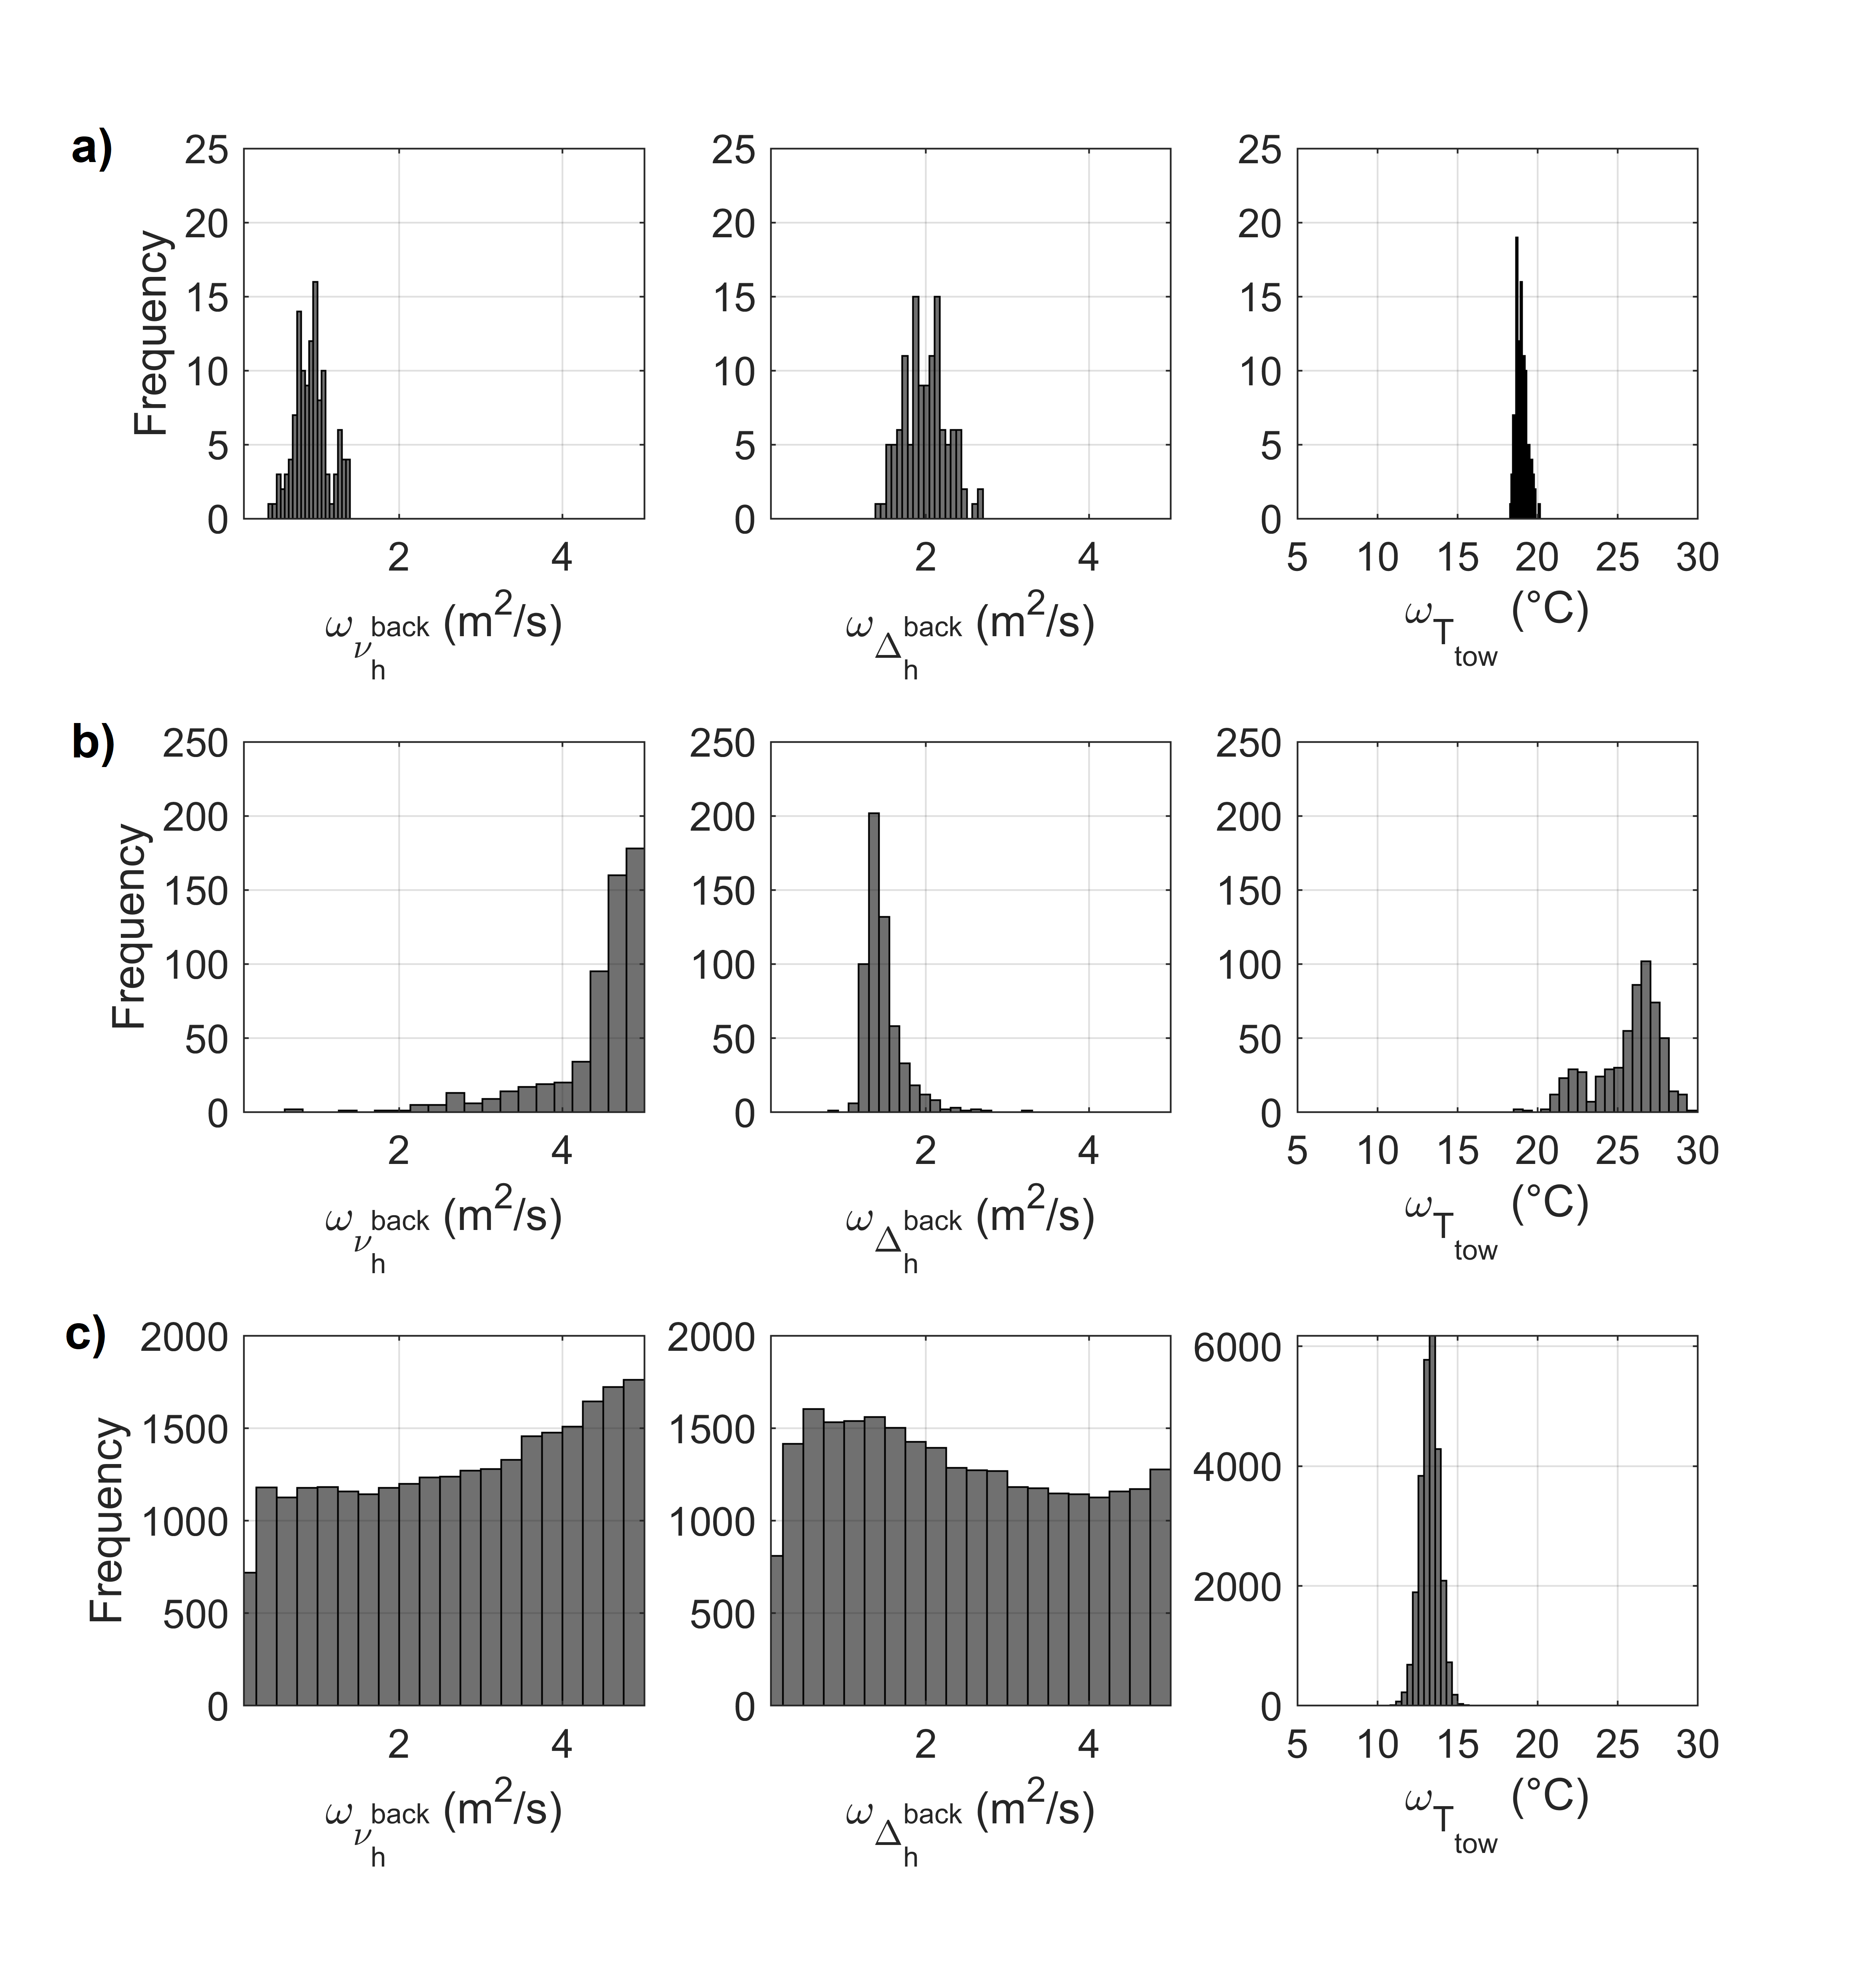
\includegraphics[width=14.5cm]{posterior_distributions.png}
	\caption{Posterior distributions of the calibration parameters after the iterative Bayesian updating in the framework of (a)~scenario~0, (b)~scenario~1, and (c)~scenario~2.}
	\label{fig03:posteriors}
\end{figure}

Figure~\ref{fig03:posteriors} thus shows how leaving out either water temperature or flow velocity measurement data increases the uncertainties of calibration results through wider, less narrow, and therefore, less assertive posterior distributions. In scenario~1, missing water temperature data leads to increased uncertainty in \(\omega_{T_{tow}}\). In scenario~2, missing flow velocity data leads to high uncertainty in \(\omega_{\nu_{h}^{back}}\) and \(\omega_{\Delta_{h}^{back}}\), which indicates that these two calibration parameters are less driven by water temperature than by flow velocity. In particular, measurements of flow velocity include patterns driven by hours of pump and turbine operation, which scenario~2 knows at its boundaries but it cannot evaluate the operation's importance to hydrodynamic patterns in the reservoir.

Fewer measurement data correspond to fewer constraints for the rejection sampling, which makes that the posterior distributions after scenarios~1 and~2 contain more samples than the more constraint scenario~0. The difference in posterior sample sizes between scenarios~1 and~2 can be explained by the higher number of velocity measurements, which makes scenario~1 more constrained than scenario~2. Therefore, Figure~\ref{fig03:posteriors} also illustrates how more calibration constraints lead to statistically more distinct calibration results.

\subsection{Maximum Likelihoods of Calibration Parameters}

% maximum-likelihood parameter values per scenario
\tablename{~\ref{tab:max_likelihood}} lists the maximum likelihoods of the calibration parameters for the three scenarios. In scenario~0, the maximum likelihoods are in a statistically reasonable range (i.e., not at the limits of the prior limits given in \tablename{~\ref{TableParam}}). However, in scenario~1, the maximum likelihood for $\nu_{h}^{back}$ is 4.83, and therefore, close to the upper limit of the prior distribution. Also, the maximum likelihood of 26.63~$^{\circ}$C for the initial water temperature is close to the upper limit of the prior distribution and physically unlikely in deeper layers of the SR. Yet, this observation is not astonishing in the absence of measurement data on the water temperature. In scenario~2, the maximum likelihoods for both $\nu_{h}^{back}$ and $\Delta_{h}^{back}$ are even closer to the upper limits of the prior distribution test ranges, which indicates that the Bayesian calibration might have gone beyond the test ranges if we had allowed it (which we have intentionally not done). Therefore, $\nu_{h}^{back}$ and $\Delta_{h}^{back}$ in scenario~2 are poorly constrained by the water temperature-only measurement data. In addition, high maximum likelihoods for $\omega_{\nu_{h}^{back}}$ and $\omega_{\Delta_{h}^{back}}$, suggest that the calibration tries to adjust the model by making diffusion a key physical process, especially in scenario~2 for achieving stratification.

\begin{table}
	\caption{Maximum-likelihood values of the calibration parameters per scenario.}
	\label{tab:max_likelihood}
	\centering
	\begin{tabular}{l l | c c c}%{P{6cm} P{3cm} | P{.75cm} P{.75cm} P{.75cm}} 
		\hline
		\multicolumn{2}{l|}{Scenario}& 0 & 1 & 2\\
		\hline
		Background horizontal eddy viscosity & $\nu_{h}^{back}$ \((m^2s^{-1})\) &  0.91 & 4.83 & 4.93 \\
		Background horizontal eddy diffusivity & \(\Delta_{h}^{back}\) \( (m^2s^{-1})\) & 2.05 & 1.38 & 4.99 \\
		Initial water temperature (intake tower)& \(T_{tow}\)   \((^{\circ} C)\) & 18.86 & 26.63 & 13.42 \\
		\hline
	\end{tabular}
\end{table}

The maximum likelihoods do not necessarily coincide with the univariate marginal peaks shown in Figure~\ref{fig03:posteriors}, which is why we look at the non-linear interdependence of the posterior distributions in the next section.

\subsection{Joint Posteriors of Calibration Parameters}

% dive into posterior dependency
The marginal posterior distributions in \figurename{~\ref{fig03:posteriors}} do not visualize the dependence between the three calibration parameters. Therefore, we show the joint posterior distributions with 3d plots in \figurename{~\ref{fig04:interdependence}}. A wide (or narrow) spread of the point cloud along a parameter's~$\omega$ axis means high (or low) uncertainty. Diagonal structures imply a linear correlation, and curved shapes indicate non-linear dependencies. The dark red color indicates the location of the maximum likelihoods listed in \tablename{~\ref{TableParam}}. For instance, comparing the location (red areas) and spread of the posterior distributions with respect to $\omega_{\nu_{h}^{back}}$ in \figurename{~\ref{fig04:interdependence}}~a and~b (scenarios~0 and 1) highlights the substantial difference in its maximum likelihood (see \tablename{~\ref{tab:max_likelihood}}).

The exclusive calibration toward water temperature data in scenario~2 (see \figurename{~\ref{fig04:interdependence}}~b and c) led to a wide spread of $\omega_{\nu_{h}^{back}}$ and $\omega_{\Delta_{h}^{back}}$, which corresponds to quasi-total independence. The spread of $\omega_{\nu_{h}^{back}}$ and $\omega_{\Delta_{h}^{back}}$ would probably have gone beyond the margins of \figurename{~\ref{fig04:interdependence}}~c, if we had also allowed physically non-meaningful value ranges. The only structure visible in \figurename{~\ref{fig04:interdependence}}~c for scenario~2 is imposed by the heavily constrained values of $\omega_{T_{tow}}$, which show the largest likelihood values in the front-right corner. This is additional (multivariate) evidence that the physically unreasonable forcing of water-temperature-driven stratification in scenario~2 caused high uncertainty regarding $\omega_{\nu_{h}^{back}}$ and~$\omega_{\Delta_{h}^{back}}$. Still, if we were only looking at the initial water temperature as a calibration parameter result, an evident misconception would be that the calibration result was good, well-constrained, and plausible.

The interdependence of calibration parameters in scenarios~0 and~1 also demonstrates that there is more than one unique parameter combination that leads to a similar model fit. Thus, the Bayesian calibration reveals the uncertainty regarding a statistically well-fitting combination of calibration parameter values (i.e., maximum likelihoods). However, also the Bayesian approach cannot generally solve the issue of equifinality as a result of weak calibration data, model simplifications, or physically non-meaningful setups. It only enables to quantify the post-calibration uncertainty (\figurename{~\ref{fig03:posteriors}} and \figurename{~\ref{fig04:interdependence}}) indicating that the calibration result is likely to be subjected to equifinality.


\begin{figure}
	\centering
	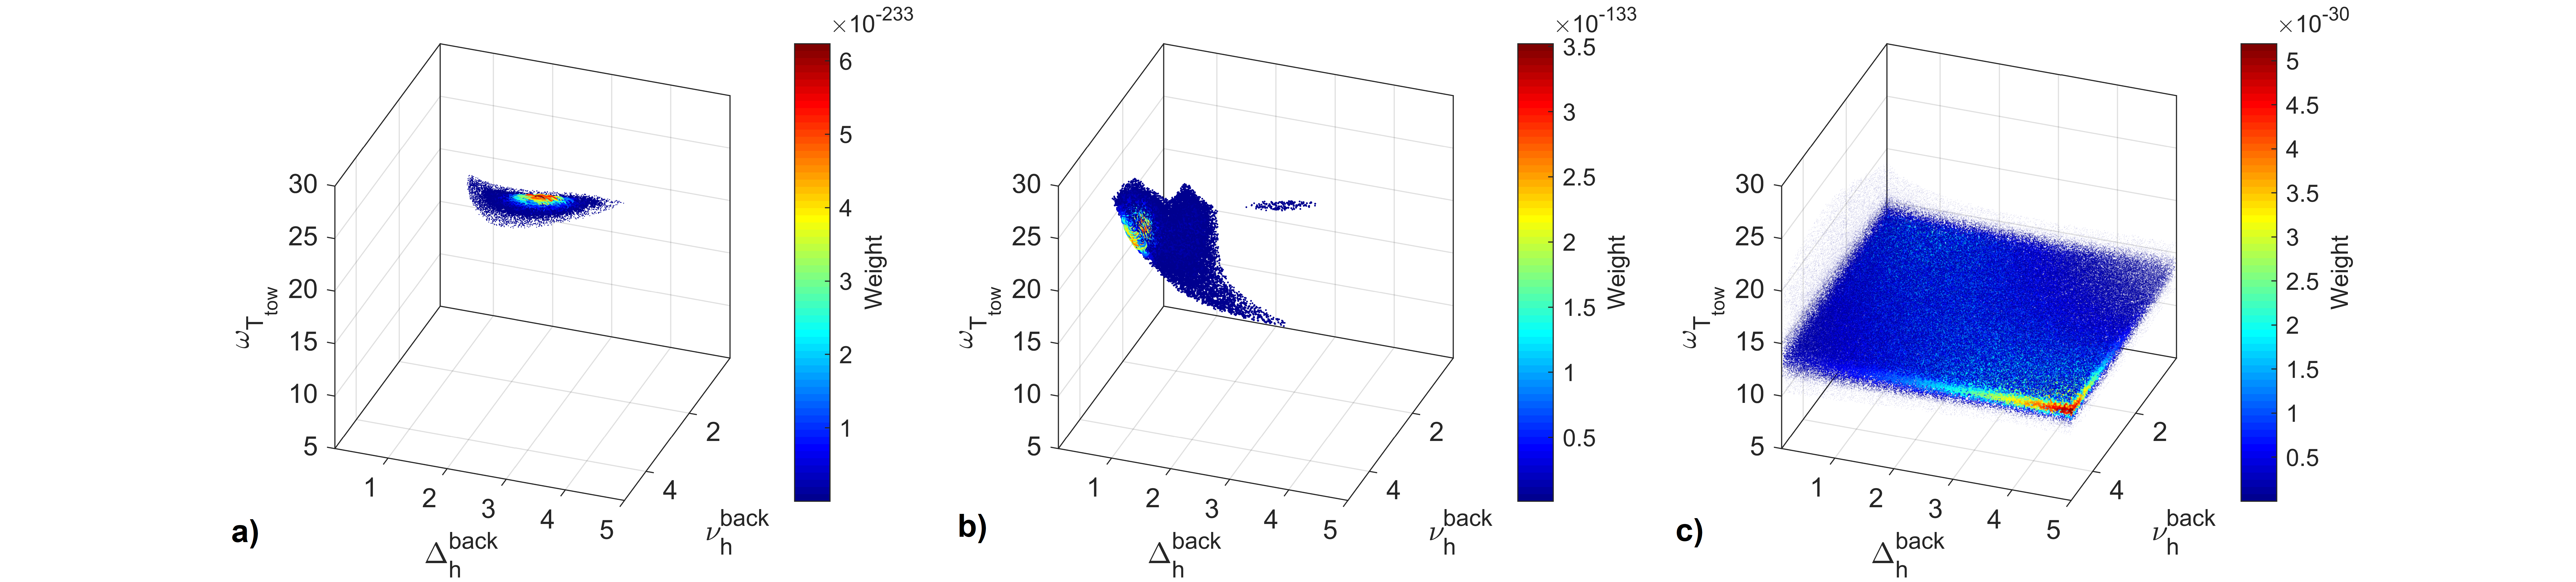
\includegraphics[width=14.5cm]{interdependence.png} % former Dependency_calibration_parameters_2
	\caption{Non-linear dependence of the calibration parameters after the last BAL iterations of (a) scenario~0,  (b) scenario~1, and (c) scenario~2.}
	\label{fig04:interdependence}
\end{figure}

\subsection{Lump-sum Statistics}

%intro an pointer to table
We ran additional simulations with both Delft3D-FLOW and the GPE-surrogate models with the maximum-likelihood calibration parameter sets resulting from the three scenarios to calculate global lump-sum statistics characterizing a generalized model quality. The resulting lump-sum statistics in the form of the mean error~\((\bar{\textit{e}})\), standard deviation from the measurements~\((\sigma_e)\), and root-mean-square error~\textit{RMSE} are listed in \tablename{~\ref{tab:model_verification}}.

\begin{table}
	\caption{Mean error~\(\bar{\textit{e}}\), standard deviation~\(\sigma_e\), and root-mean-square error~\textit{RMSE} of the calibrated full-complexity and GPE-surrogate model runs with the maximum likelihoods of the calibration parameters after the three scenarios.}
	\label{tab:model_verification}
	\centering
	\begin{tabular}{P{2cm} l c c c c} 
		\hline
		Model & Parameter & Scenario & \(\bar{\textit{e}}\) & \(\sigma_e\) & \textit{RMSE}\\
		\hline
		\multirow{4}{4em}{Delft3D-FLOW} & \multirow{2}{2em}{$U$~(mm~s$^{-1}$)} & 0 & 0.44 & 2.53 & 2.56 \\
		\cline{3-6}
		& & 1 & 0.19 & 1.42 & 1.43\\
		\cline{2-6}
		& \multirow{2}{2em}{$T$~(\(^{\circ}\)C)} & 0 & -3.67 & 3.84 & 5.24\\
		\cline{3-6}
		& & 2 & 0.16 & 1.80 & 1.76\\
		\hline
		\multirow{4}{4em}{GPE-surrogate} & \multirow{2}{2em}{$U$~(mm~s$^{-1}$)} & 0 & 0.31 & 1.41 & 1.44 \\
		\cline{3-6}
		& & 1 & -0.03 & 1.25 & 1.24\\
		\cline{2-6}
		& \multirow{2}{2em}{$T$~(\(^{\circ}\)C)} & 0 & -3.77 & 3.85 & 5.31\\
		\cline{3-6}
		& & 2 & 0.14 & 1.79 & 1.75\\
		\hline
	\end{tabular}
\end{table}

% flow velocities RMSE in scenario 0
In the all-data scenario~0, the \textit{RMSE} regarding the depth-averaged flow velocity $U$ in Delft3D-FLOW is 2.56~mm~s\textsuperscript{-1}, which represents a 17\%-deviation compared with the time-averaged measurement data. One reason for the $U$~deviations is the weaknesses in reproducing the magnitude and timing of peaks that stem from pump and turbine operations. The GPE-surrogate model reproduced the data slightly better, with a smaller \textit{RMSE} of 1.44~mm~s\textsuperscript{-1} and a slightly better representation of peaks in magnitude and time. This slightly better performance of the GPE indicates an imperfect surrogate approximation, as the maximum likelihood parameter sets identified with the GPE perform slightly less well when plugged into the full-complexity Delft3D-FLOW model. However, in light of the standard deviation of measurement errors of the flow velocity measurements (3~mm~s\textsuperscript{-1}), the \textit{RMSE}s represent an excellent performance of both models after scenario~0.


\subsection{Bayesian Calibration Residuals and Posterior Predictions}

The modeled $U$ and $T$ with the maximum likelihoods of the calibration parameters also enable us to evaluate the model improvement through the Bayesian calibration. For this purpose, we additionally consider the model residuals, here defined as the vertical (flow velocity) or horizontal (water temperature) distances between the measured and simulated values. 

\figurename{~\ref{fig05:postU}}~a and~b illustrate the depth-averaged flow velocity~$U$ at the measurement station for scenarios~0 and~1 (i.e., the two scenarios considering flow velocity measurements). The blue lines are the results of the Delft3D-FLOW (closed blue line) and surrogate (dashed blue line) models with the maximum likelihoods (\tablename{~\ref{tab:max_likelihood}}). The gray lines are the results of the training runs, which constitute the standard deviation (uncertainty) of the posterior distributions (Figure~\ref{fig03:posteriors}). In addition, the closed black lines show the depth-averaged flow velocity measurements and enable us to identify the model residuals (i.e., vertical differences with the model results).

The posterior surrogate model outputs well fit the measurement data with small residuals after both scenarios. In addition, the posterior time-averages of $U$ are 1.65~mm~s\textsuperscript{-1} and 1.05~mm~s\textsuperscript{-1} in scenarios~0 and~1, respectively. Thus, the calibration with flow velocity data yielded small calibration errors (i.e., residuals), which are close to zero on average. The calibration also reduced the model uncertainty in both scenarios, with, for instance, the time-averaged standard deviation in scenario~1 decreasing from 12.1~mm~s\textsuperscript{-1} (prior according to \tablename{~\ref{TableParam}}) to 0.4~mm~s\textsuperscript{-1} (posterior).

A comparison of the two scenarios~0 and~1 shows that the models perform especially better in scenario~1 regarding the magnitude and time of flow velocity peaks. In particular, after scenario~1, both models well simulate the shape and magnitudes of the measurement data, although with too small amplitudes of local extrema (lows and peaks). The improved accuracy after scenario~1 is also reflected in \textit{RMSE}s of 1.43~mm~s\textsuperscript{-1} (Delft3D-FLOW) and 1.24~mm~s\textsuperscript{-1} (GPE-surrogate), which are both smaller than after scenario~0 (see also \tablename{~\ref{tab:model_verification}}). Already Figure~\ref{fig03:posteriors} indicated that the flow velocity data have higher importance for the hydrodynamic patterns in the reservoir than the water temperature measurements (differences between Figure~\ref{fig03:posteriors}~b and~c). Figure~\ref{fig05:postU} confirms this observation by indicating that the water temperature data in scenario~0 lead to a worse replication of flow velocity measurements. The reason is that in scenario~0, the calibration had to meet two measurement targets that compete with each other due to imperfect model assumptions (i.e., too short time for stratification).

\begin{figure}
	\centering
	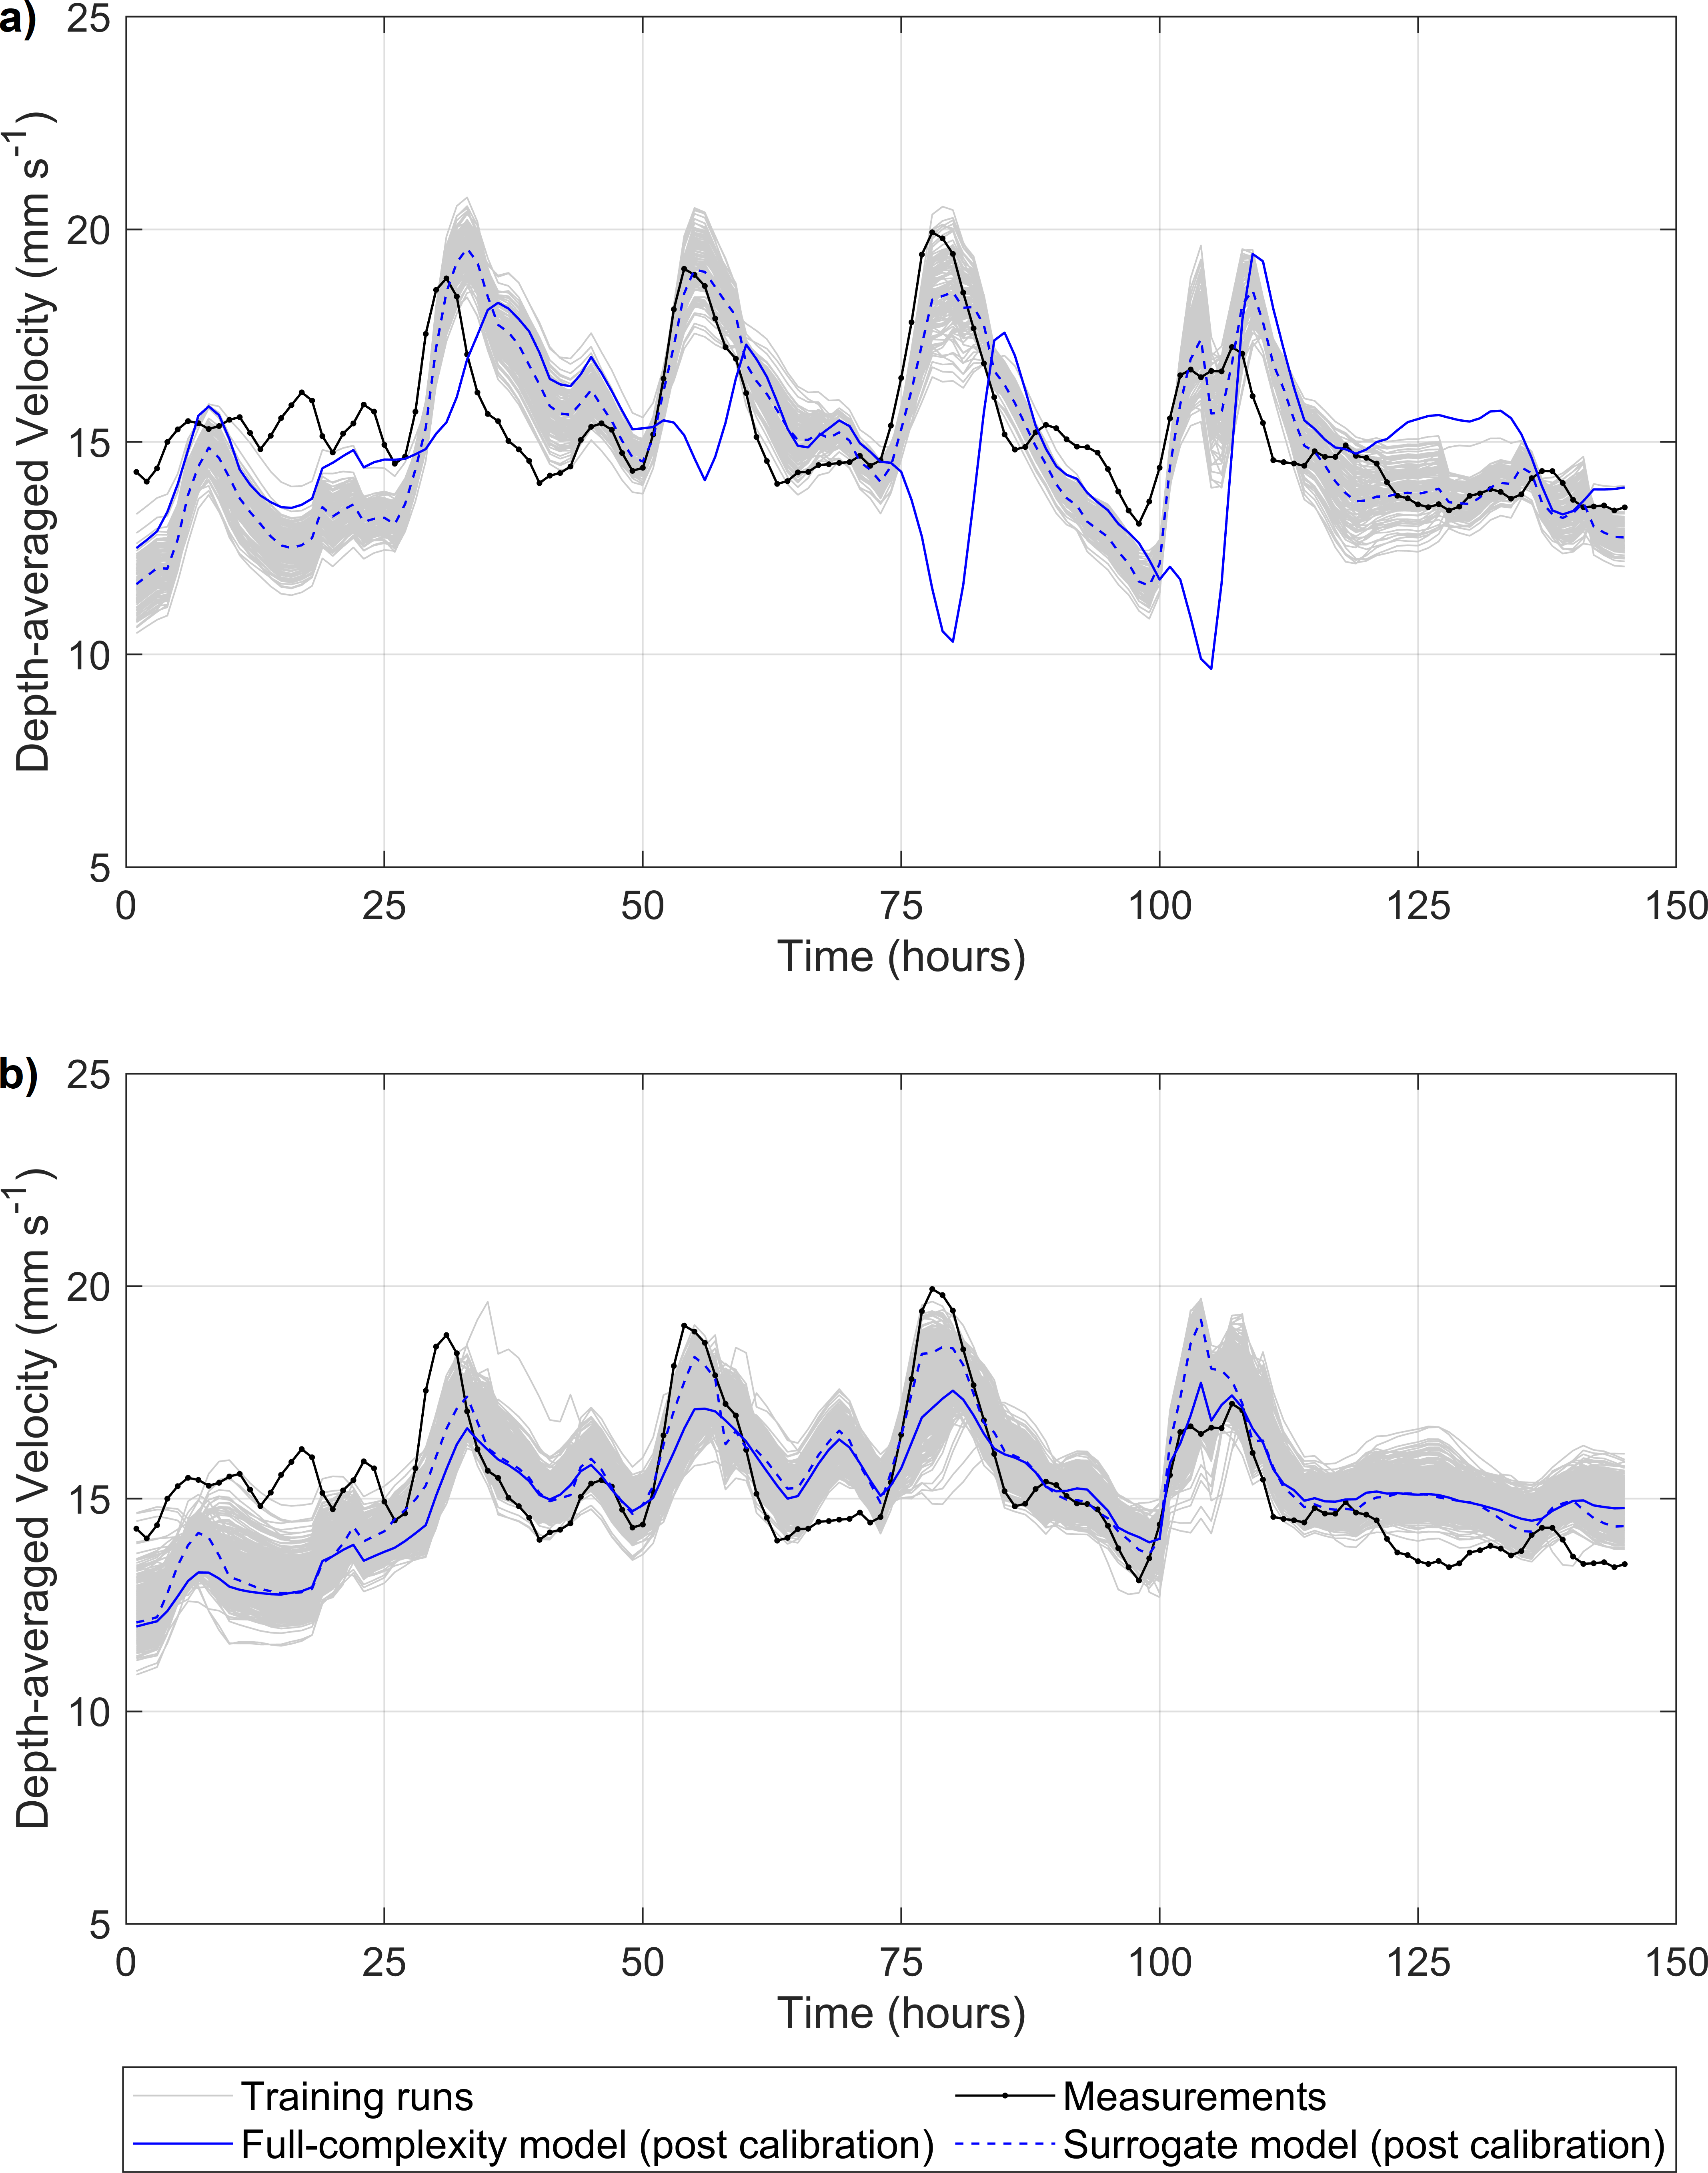
\includegraphics[width=14.5cm]{post-U-xscenario.png} 
	\caption{Simulated depth-averaged horizontal flow velocity~$U$ resulting from (a) scenario~0 and (b) scenario~1 in the considered period from August~1 (00:00~AM) through August 7 (00:00~AM), 2016. The graphs correspond to the location of the measurement station in the reservoir and feature results of the training runs, surrogate model, and full-complexity Delft3D FLOW model in addition to the measurements.}
	\label{fig05:postU}
\end{figure}

\figurename{~\ref{fig06:postT}}~a and~b show the water temperature profiles~$T$ at the measurement station for scenarios~0 and~2 (i.e., the two scenarios considering water temperature data). The blue lines are the results of the Delft3D-FLOW (closed blue line) and surrogate (dashed blue line) models with the maximum likelihoods (\tablename{~\ref{tab:max_likelihood}}). The gray lines are the results of the training runs, which constitute the standard deviation (uncertainty) of the posterior distributions (Figure~\ref{fig03:posteriors}). In addition, the closed black lines show the depth-averaged flow velocity measurements and enable us to identify the model residuals (i.e., vertical differences with the model results).

In scenario~0, the calibration was forced to compromise between fitting the water temperature and flow velocity data, which is reflected in the physical weaknesses of the results. For instance, the water temperature profile modeled with the posterior maximum likelihoods is close to constant over depth and far away from the measurement data. Thus, the calibrated model fails to reproduce the temperature stratification in the all-data scenario~0, which makes sense because of the too-short time frame for the onset of stratification. In addition, in scenario~0, the residuals of the prior and posterior model outputs have considerably high averages of 3.58\(^{\circ}\)C and 4.93\(^{\circ}\)C, respectively.

After scenario~2, the modeled posterior water temperature profiles show smaller residuals (i.e., it is generally closer to the measurements) than the prior profiles. The posterior profile also shows signs of temperature stratification, with water temperatures at the surface approximately 1$^{\circ}$C higher than in deeper layers. The better simulation of water temperature profiles also reflects in the \textit{RMSE} (\tablename{~\ref{tab:model_verification}}) reducing from 5.3$^{\circ}$C in scenario~0 to 1.75\(^{\circ}\)C in scenario~2. Therefore, scenario~2 also performs better in terms of lump-sum statistics regarding $T$ than scenario~0. However, the fast stratification achieved in scenario~2 is physically unlikely, and thus, represents a poor calibration even though the lump-sum statistics (\tablename{~\ref{tab:model_verification}}) suggest good model performance. Thus, considering exclusively water temperature measurements in scenario~2 led to improved simulation of water temperature measurements, although the water temperature profile still does not correspond well to the measurements.

\begin{figure}
	\centering
	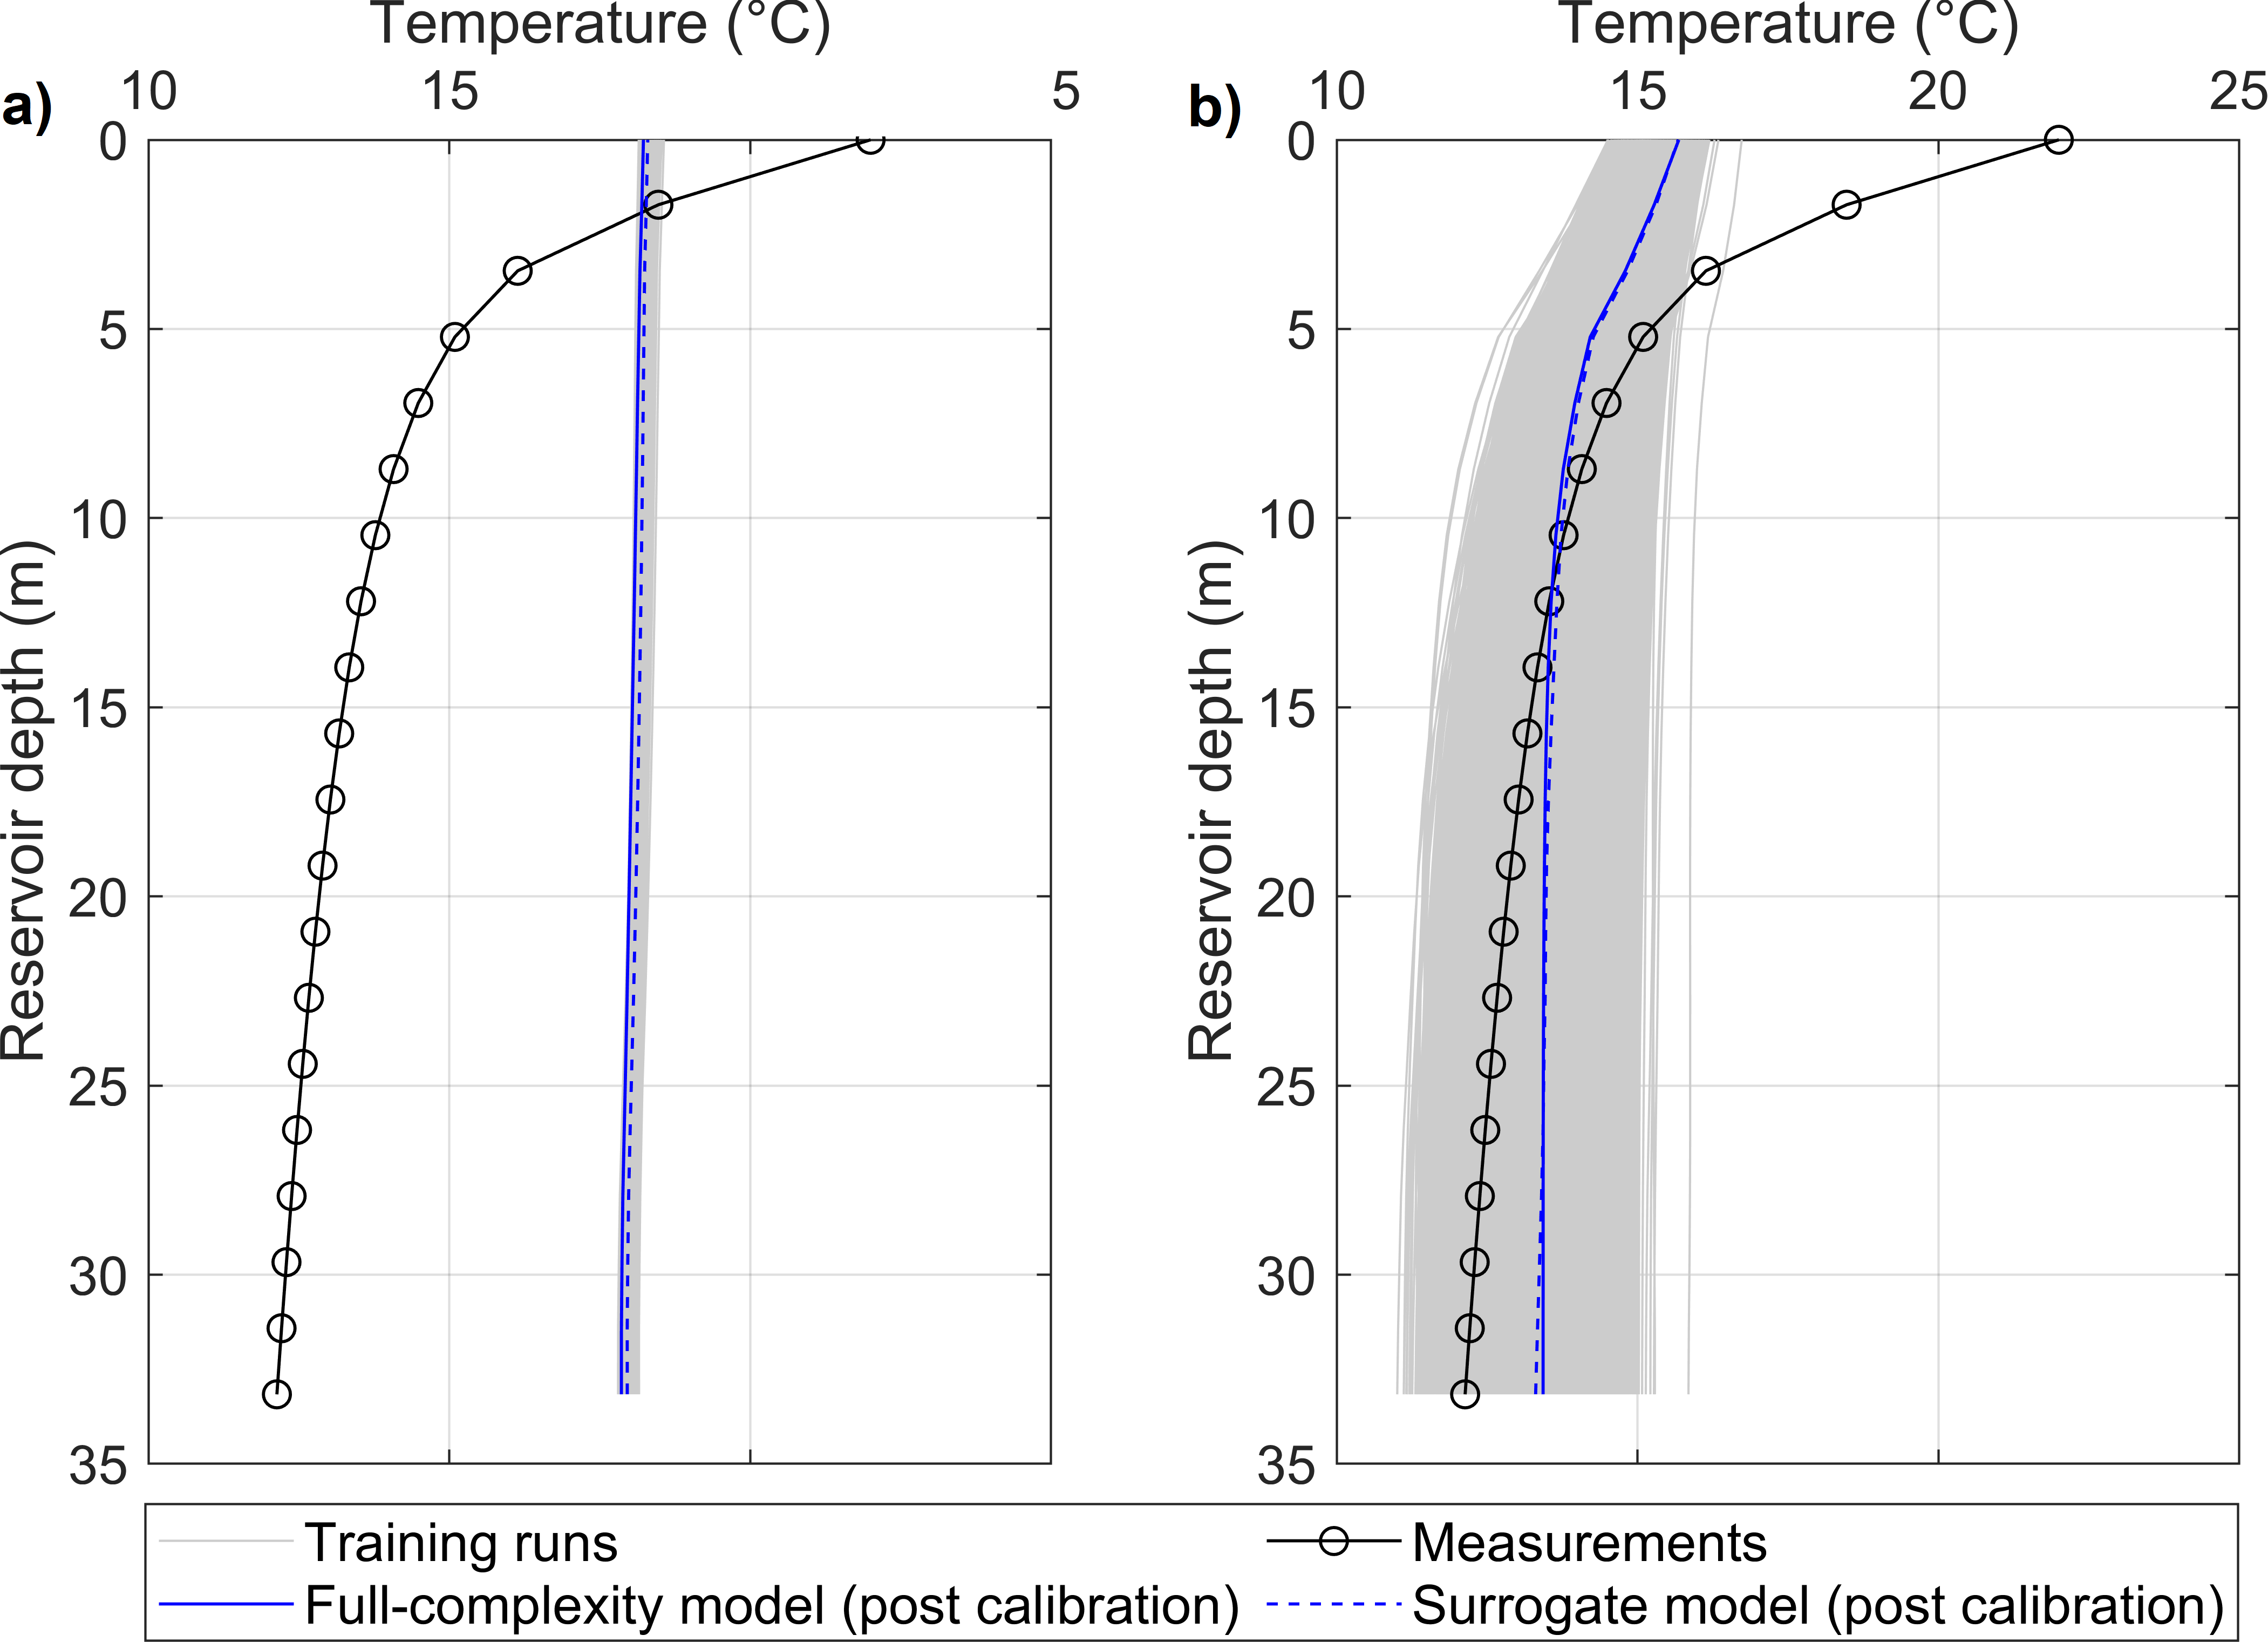
\includegraphics[width=10cm]{post-T-xscenario.png} % former: Temp_PriorPosterior_FirstStage_ThirdStage
	\caption{Simulated water temperature~$T$ profiles resulting from (a) the scenario~0 and (b) the scenario~2 calibrations at the measurement station. The graphs show the results of the training runs, surrogate model, and full-complexity Delft3D-FLOW model in addition to the measurements.}
	\label{fig06:postT}
\end{figure}

These observations show that scenario~0 simulates flow velocities better than water temperature. Still, scenario~0 simulates flow velocities less correctly than scenario~1, which does not know the water temperature data. Because pump and turbine operations are the main drivers for fluxes in the SR, the higher importance of flow velocity measurements indicates that hydrodynamic patterns are only secondarily controlled by heat-driven stratification.


% --- END OF RESULTS ACCORDING TO THE TEST PROCEDURE SECTION ---

\section{Discussion}

\subsection{Physical Relevance}

Figures~\ref{fig07:turbine} and~\ref{fig08:pump} map horizontal (non-depth-averaged) flow velocity calculated with the calibrated full-complexity Delft3D-FLOW and GPE-surrogate model. The maps show flow velocity magnitudes (not directions) in the entire SR during turbine and pump operation hours, respectively, and with the maximum likelihoods from the all-data scenario~0. The turbine operation map (Figure~\ref{fig07:turbine}) represents a model snapshot on August~2, 2016, at 10:00~PM, and the pump operation map (Figure~\ref{fig08:pump}) represents a snapshot on August~3, 2016, at 03:00~AM. Both figures show the horizontal flow velocity magnitudes at different water depths of 3~m, 16~m, and 30~m below the maximum operation water level (668.5~m~a.s.l.). The pump and turbine operation hours are particularly interesting in light of the above observations because they potentially counteract stratification. 

% turbine operation
In the case of turbine operation (\figurename{~\ref{fig07:turbine}}), the calibrated GPE-surrogate (\textit{GPE$_{Adjusted}$} in the plots) and full-complexity models show two currents in the reservoir center and near the dam at depths of 3~m and 16~m. Those currents can be related to the inflows from the conveyance tunnel that is located at the South-West shore, approximately 400~m upstream of the dam (see also \figurename{~\ref{fig:sr_map}}). The highest flow velocities occur in the vicinity of the dam where turbine operation draws water from the reservoir.

% pump operations
The pump operations in \figurename{~\ref{fig08:pump}} show a similar pattern, but with inverse velocity vector directions (directions are not visible on the magnitude maps). At a water depth of 16~m, both turbine and pump operations form a large eddy pattern in the reservoir with slow horizontal flow velocities that might affect the stratification of the water temperature.

While scenario~0 replicates flow velocity at the measurement station acceptably well (Figure~\ref{fig05:postU}), it does not well reproduce temperature-driven stratification (Figure~\ref{fig06:postT}), supposedly because pump and turbine operations outweigh stratification. Also, the maps of the horizontal flow velocity magnitudes (not directions) in \figurename{~\ref{fig07:turbine}} and \figurename{~\ref{fig08:pump} show that turbine and pump operations have a great influence on the reservoir hydrodynamics. That is, the primary importance for reservoir hydrodynamics in the presence of pump and turbine operations is measured flow velocity, which is in line with observations in other studies \cite{muller_flow_2018}. Still, the high values for $\omega_{\nu_{h}^{back}}$ and $\omega_{\Delta_{h}^{back}}$ (\tablename{~\ref{tab:max_likelihood}}), especially after scenario~2, indicate that the Bayesian calibration is trying to make diffusion a key process. However, the dominance of pump- and turbine-driven flow velocity patterns rather suggest that advection is the real key process.

The \textit{RMSE}s of the calibrated GPE-surrogate and the full-complexity models, lump-summed over the entire simulation period, are small (cf.~\tablename{~\ref{tab:model_verification}}), but do not show the spatiotemporal variation that can be seen in Figures~\ref{fig07:turbine}} and~\ref{fig08:pump}. Thus, the \textit{RMSE}s compared with the absolute magnitudes suggest that the stochastic calibration yielded very good global model statistics, even though scenario~0 is a physical compromise that necessarily involves the wrong replication of flow velocity and water temperature patterns. In consequence and in light of Figures~\ref{fig05:postU} and \ref{fig06:postT}, the horizontal flow velocity magnitude maps indicate that the small global errors may hide high errors at a detailed scale where local errors potentially cancel each other.

\begin{figure}
	\centering
	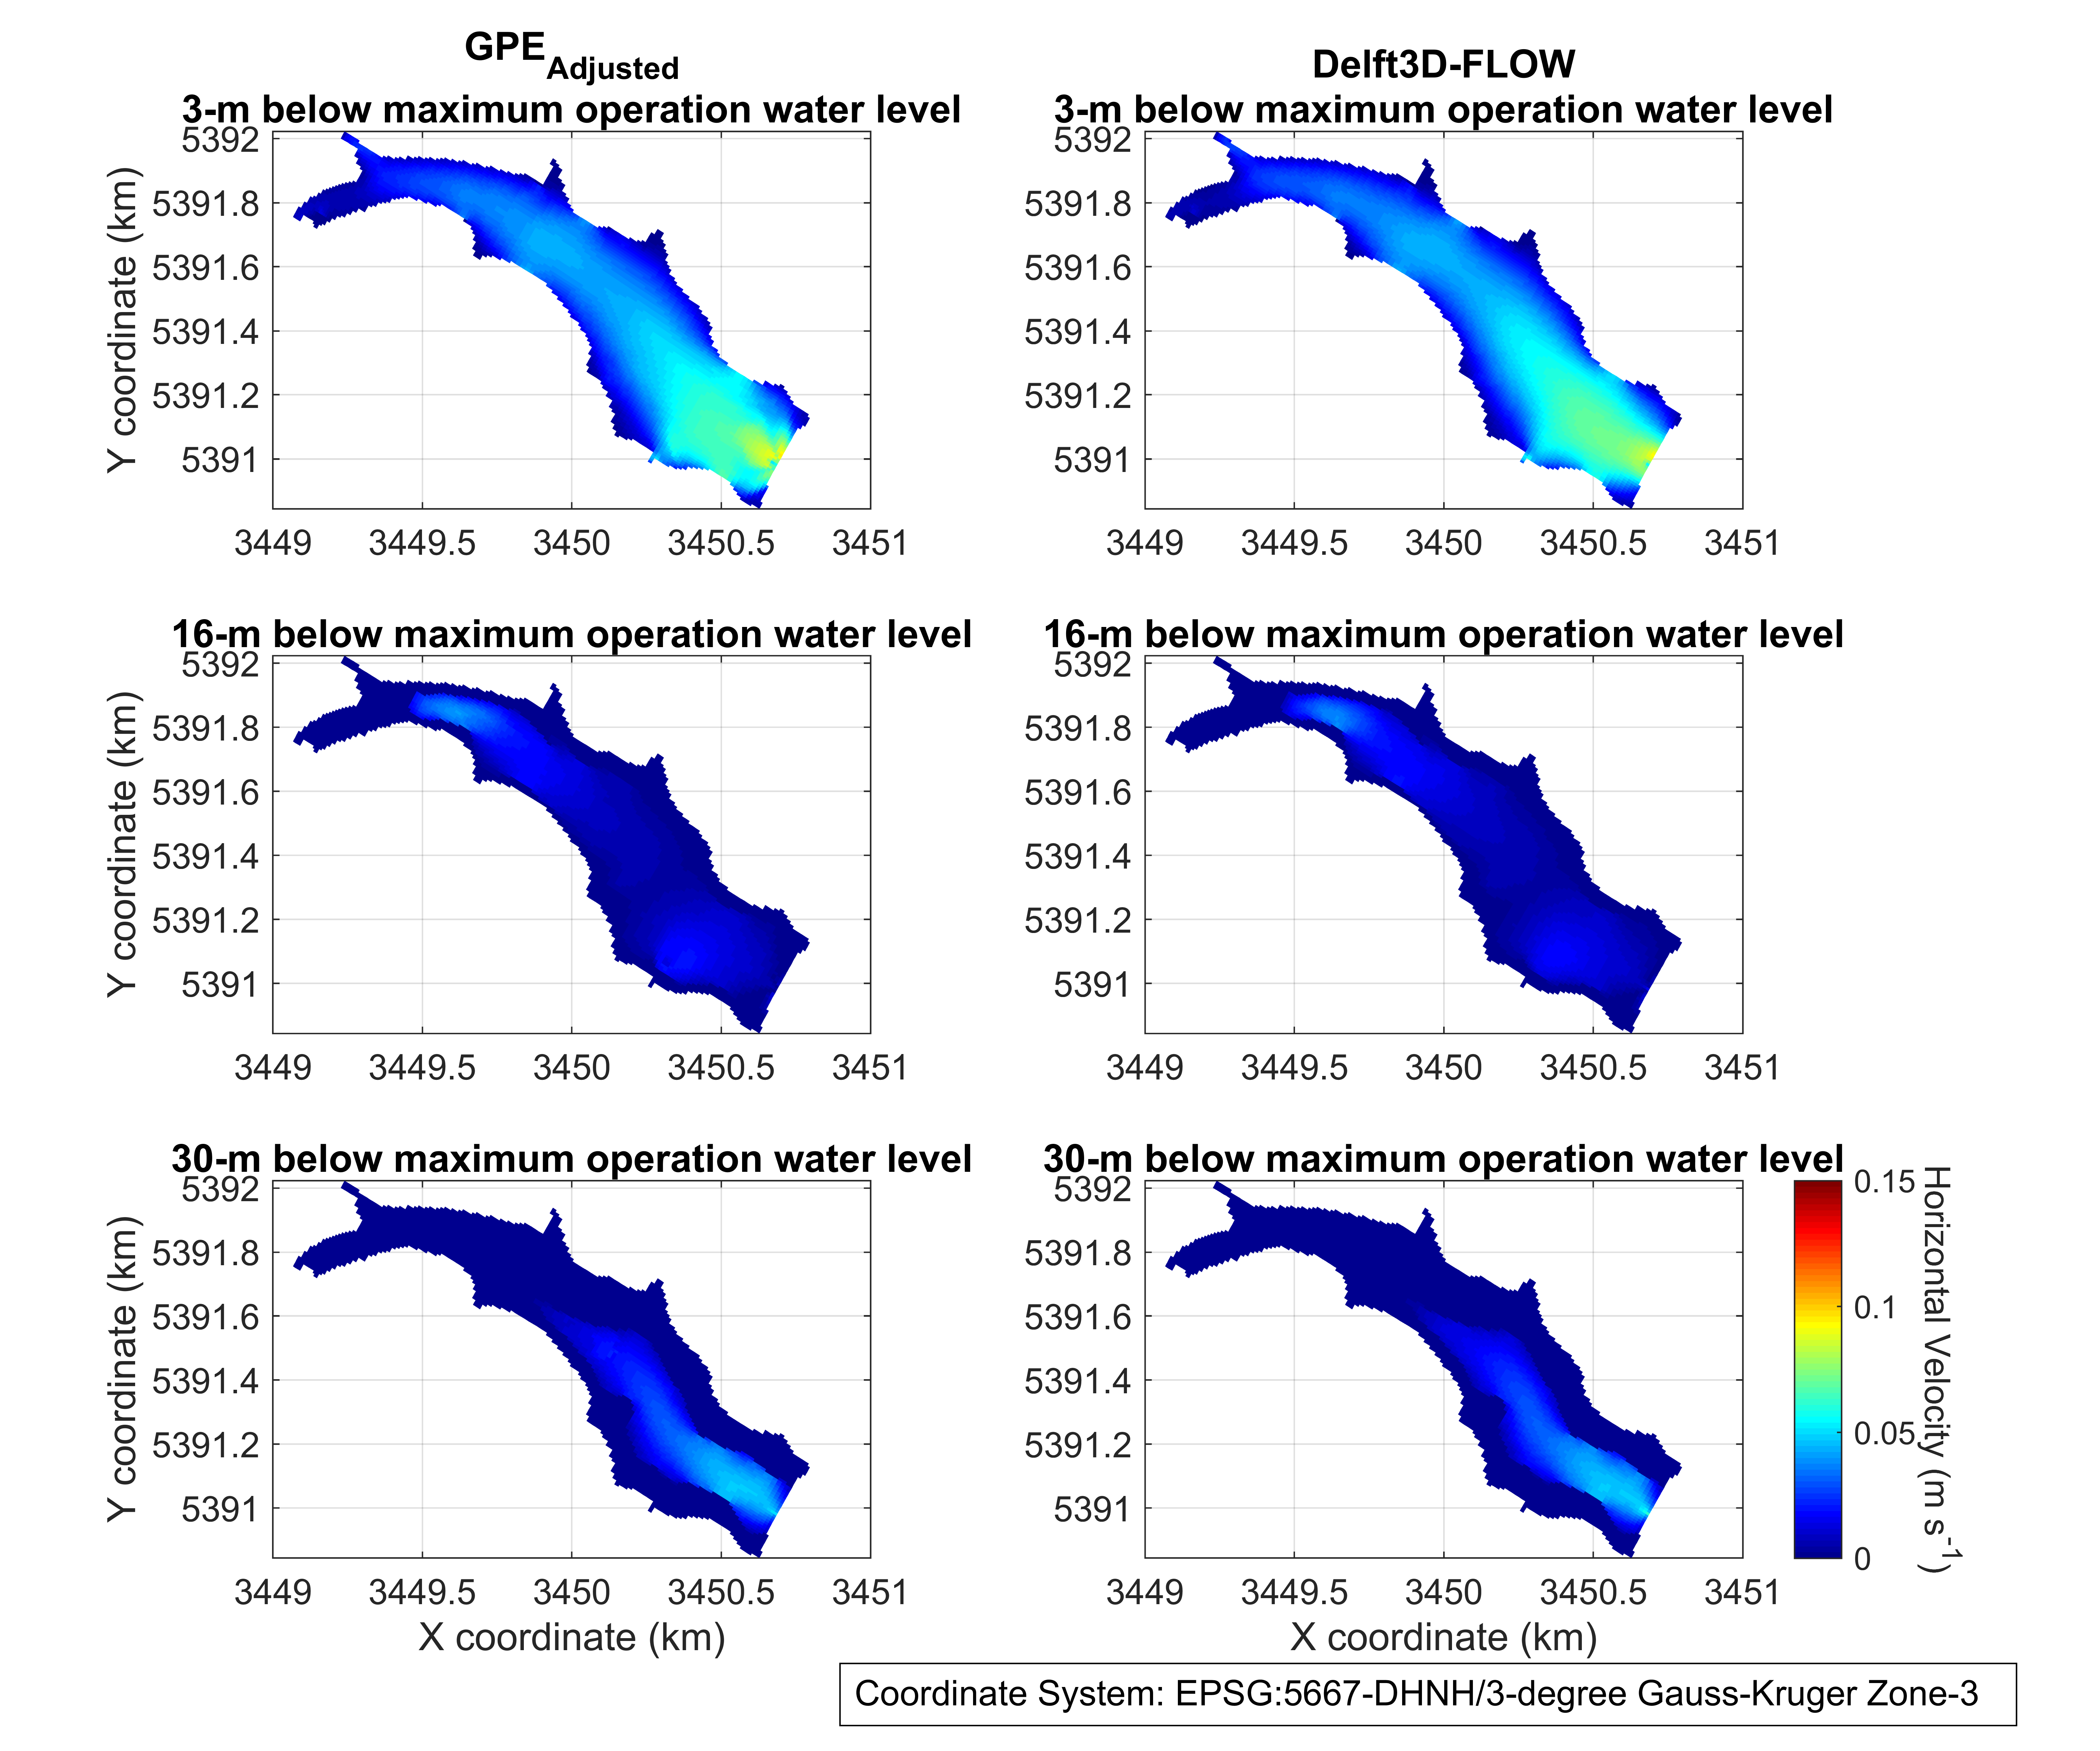
\includegraphics[width=16cm]{turbine.png}
	\caption{Horizontal flow velocity magnitudes in the reservoir at 3~m (top row), 16~m (middle row), and 30~m (bottom row) below the water surface during turbine operation (on August 2, 2016, at 10:00~PM). The results are produced with the calibrated GPE (\textit{GPE$_{Adjusted}$}) and Delft3D-FLOW model using the maximum likelihoods of calibration parameters according to scenario~0.}
	\label{fig07:turbine}
\end{figure}

\begin{figure}
	\centering
	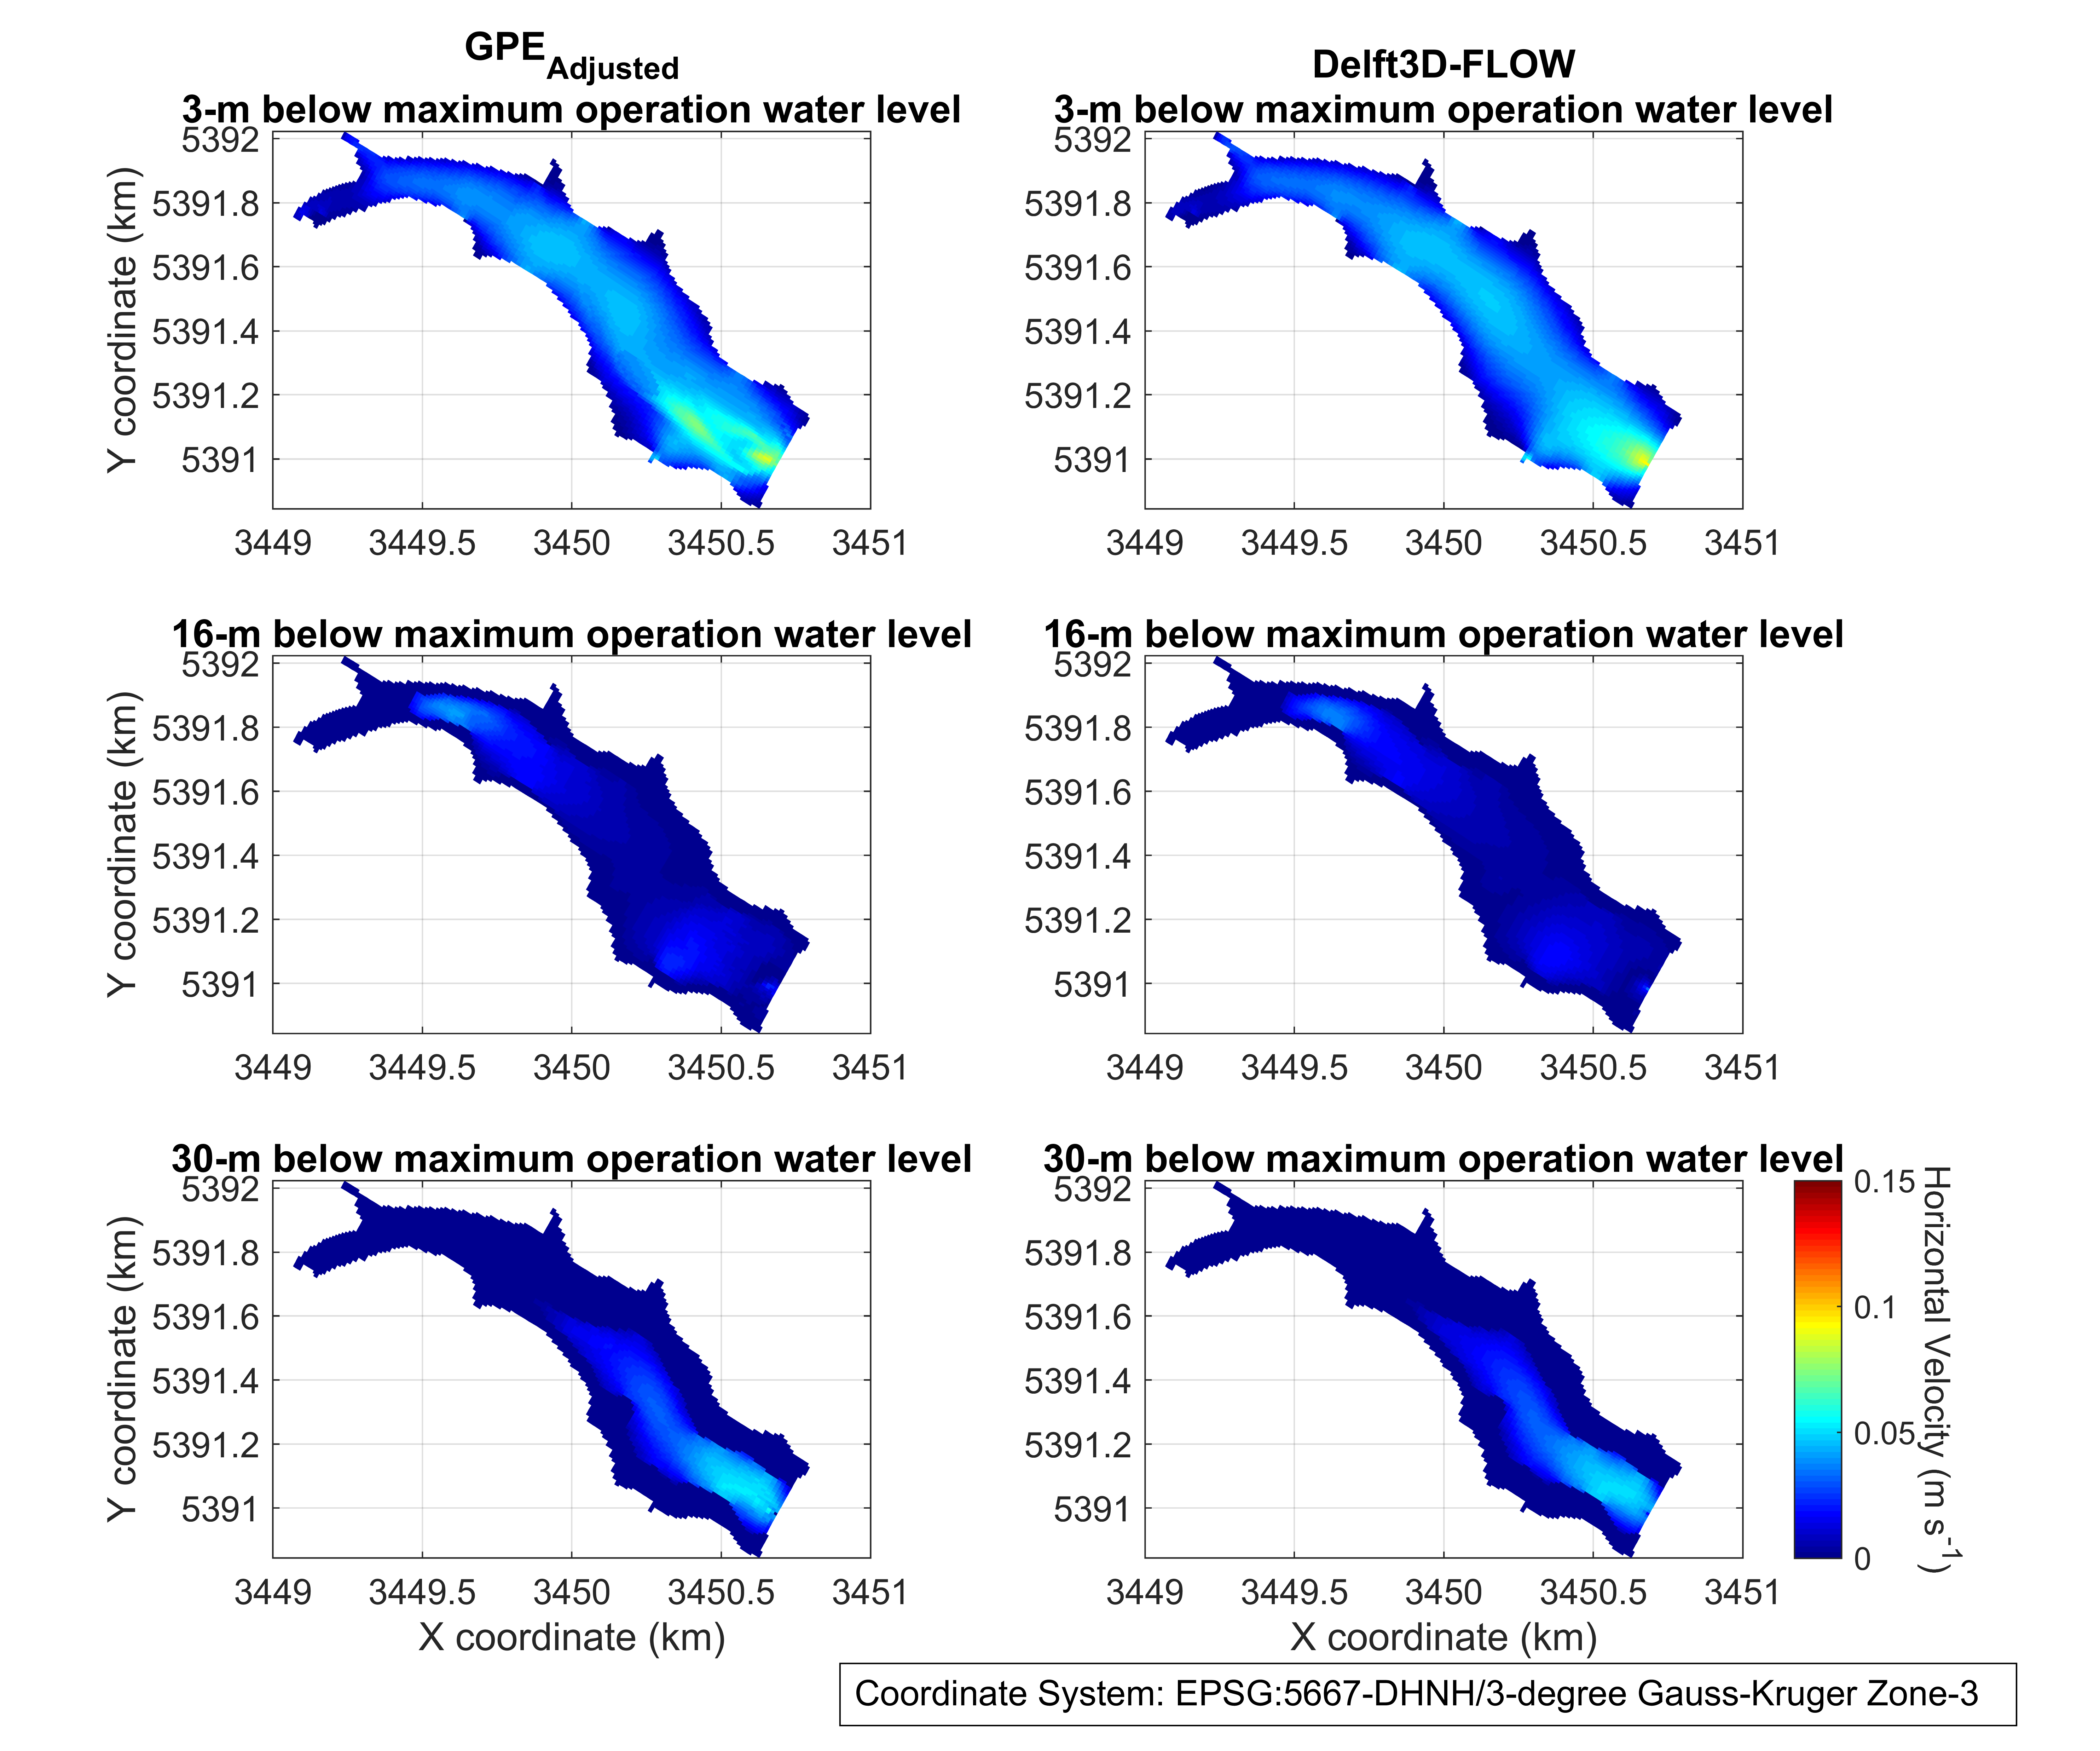
\includegraphics[width=16cm]{pumping.png}
	\caption{Horizontal flow velocity magnitudes in the reservoir at 3~m (top row), 16~m (middle row), and 30~m (bottom row) below the water surface during pump operation (on August 3, 2016, at 03:00~AM). The results are produced with the calibrated GPE (\textit{GPE$_{Adjusted}$}) and Delft3D-FLOW model using the maximum likelihoods of calibration parameters according to scenario~0.}
	\label{fig08:pump}
\end{figure}


\subsection{Efficiency of Bayesian Calibration with a GPE-Surrogate Model}

% internal note: if we need to shorten, we can push this subsection to the supplemental parameters, too
The Bayesian calibration yielded statistically high global model accuracy in terms of \textit{RMSE} (see \tablename{~\ref{tab:model_verification}}), and the GPE-surrogate model increased computational efficiency almost by a factor of~10$^6$. Thus, the trained GPE-surrogate model enabled us to test as many as 10$^6$ parameter sets in the Monte-Carlo rejection sampling. In addition, the GPE-surrogate model reproduced the outcomes of the original model reasonably well and even outperformed the full-complexity model in some cases (see statistics in \tablename{~\ref{tab:model_verification}}), which is in line with other studies using Bayesian calibration \cite<e.g.,>{beckers_bayesian_2020}. The better performance of the surrogate model is possible because its training builds on the results of the numerical model and measurement data. Still, the surrogate model can only mimic a snapshot state of the numerical model (e.g., the end of the simulation), not physical processes. Thus, the surrogate model cannot write results at a specific point in time, for example, during turbine or pump operation hours.

\subsection{Choice of Calibration Parameters and Data}

While the background horizontal eddy viscosity~$\nu_{h}^{back}$ and diffusivity~$\Delta_{h}^{back}$, as well as the initial water temperature~$T_{tow}$ were chosen as constraining calibration parameters, there are many other unconstrained (constant) parameters. We made and had to make simplifications about environmental processes, which are necessary for modeling hydrodynamics of pump-storage reservoirs \cite{bermudez_res_2018, encinas_fernandez_diurnal_2020,salehi_delft3d_2017}. Other factors influencing lake stratification could be, for instance, biotic parameters such as nutrients, carbon, or oxygen concentration \cite{chanson_disp_2004}. The importance of these factors can be considered small in this study because they are primarily relevant for long-term, multi-year processes \cite<e.g., climate change predictions, cf.>{wahl_effect_2014,woolway_2021}. However, other external physical factors, such as solar radiation and wind, are likely to have affected the measurements, but we did not consider their calibration. For instance, we did not consider the adaptation of model parameters accounting for potentially cooling precipitation \cite{zhang_thermal_2020} and assumed the meteorological conditions for stratification \cite<e.g., defined in>{bermudez_res_2018,salehi_delft3d_2017} as measured deterministic constants even though we interpolated them from a measuring station located 22~km away from the reservoir. The calibration of external meteorological parameters could additionally influence the lake stratification, but it would only be another possibility to achieve physically unlikely fast lake stratification within 6~days. For testing our hypotheses, however, it was sufficient to only calibrate reservoir-internal hydrodynamic parameters, where the environmental boundary conditions needed to allow for lake stratification. Ultimately, we emulated physically more reasonable boundary conditions for testing our hypotheses without calibrating parameters other than $\nu_{h}^{back}$, $\Delta_{h}^{back}$, and~$T_{tow}$.

% consequences of this finding for the practice
To broaden the range of validity of a reservoir model, the number of calibration parameters and measurement quantities (i.e., the number of columns in $\mathbf{D}$) should be possibly high. In this context, the number of measurements per quantity (i.e., the number of rows in $\mathbf{D}$) is less important where at least 20 training measurements per quantity were already enabled calibration toward water-temperature measurements, even though it was physically wrong. Thus, for a more holistic replication of system processes, more and different measurement quantities are better than more measurements per quantity at a single location. For instance, it was better to have multiple measurement devices to collect data about different quantities with a smaller number of measurements per device (quantity), rather than using only one measurement device to get a high number of measurements of one quantity only. Still, if a measurement quantity is influenced by the local environment, sufficient measurements should be recorded in every sub-environment. For instance, velocity measurement in a reservoir should be made in fast-flowing regions at the shallow reservoir head, and slow-flowing shallow regions (i.e., the shoreline) as well as in deep regions (center of the reservoir).

\subsection{Effects of Varying Measurement Data Usage (Hypothesis~(i))}

% unpack hypothesis i
The first hypothesis~(i) was that a hydrodynamic model of a reservoir can correctly reproduce measurement data with calibration parameter combinations that are physically not meaningful. For instance, Reynolds-averaging in numerical simulations is known to result in physically non-meaningful representations of 3d flow characteristics, such as negative eddy viscosity \cite{booij_measurements_2003}. To test hypothesis~(i) in light of Bayesian calibration, we first consider the global statistics in \tablename{~\ref{tab:model_verification}} with respect to the three scenarios and their varying calibration constraints through the number of measurement quantities involved.

% evaluate the difference of using either dataset
The \textit{RMSE} of depth-averaged horizontal flow velocities~$U$ is considerably smaller when calibrated with flow velocity data only (scenario~1) than when calibrated with both water temperature~$T$ and $U$ in the all-data scenario~0. Likewise, the \textit{RMSE} of water temperature~$T$ is substantially smaller when calibrated with water temperature data only (scenario~2) than when calibrated with both $T$ and $U$ in scenario~0. Thus, the water temperature data \emph{statistically} improved calibration accuracy, even though scenario~2 was designed to be physically the most unreasonable. In this light, the lump-sum statistics in \tablename{~\ref{tab:model_verification}} suggest that adding information on either quantity improved the model quality more than adding information on both quantities. To unpack this observation, we recall the comparisons of measured and modeled $U$ in \figurename{~\ref{fig05:postU}} and $T$ in \figurename{~\ref{fig06:postT}} at the measurement station. Both quantities ($U$ and $T$) are represented physically worse when the measurement data lead to contradicting adaptation trends of the three calibration parameters. For instance, the Bayesian calibration (cf.~\tablename{~\ref{tab:max_likelihood}}) suggests that the maximum likelihood for initial water temperature $T_{tow}$ is 26.63$^{\circ}$C when the flow velocity measurement data only was considered and 13.42$^{\circ}$C when water temperature measurement data only was considered. When both measurement quantities were considered, the maximum likelihood is 18.86$^{\circ}$C (i.e., somewhere between the single-quantity considerations).

A similar observation can be made regarding the background horizontal eddy diffusivity~$\Delta_{h}^{back}$. However, the combination of the somewhere-in-the-middle compromises for the maximum likelihoods of ${T_{tow}}$ and~${\Delta_{h}^{back}}$ led to a maximum likelihood of background horizontal eddy viscosity~${\nu_{h}^{back}}$ of 0.91, which is very different than the single measurement data considerations that resulted in 4.81 and 4.93 in scenarios~1 and~2, respectively. An explanation for the differences in the ${\nu_{h}^{back}}$ maximum likelihoods is that the scenarios~1 and~2 fitted toward $U$ and $T$ based on $U$ and $T$ data only and respectively. Still, calibration with both $U$ and $T$ data resulted in the globally most robust model calibration (e.g., as indicated in the parameter interdependence plots in \figurename{~\ref{fig04:interdependence}}), compared with using either $U$ or $T$, even in the case of physically more unlikely conditions.

Thus, to mimic the measurement data, the calibration process in the $T$-only scenario~2 determined values for $\nu_{h}^{back}$ and $\Delta_{h}^{back}$ that are close to the upper limits of the physically relevant calibration ranges (\tablename{~\ref{TableParam}} compared with \tablename{~\ref{tab:max_likelihood}}) and subjected to high uncertainty (Figure~\ref{fig03:posteriors}). This perfection comes at the expense of unconstrained parameters that are not reflected in the measurement data. For instance, the exclusive consideration of water temperature measurements in scenario~2 made that $T$ is well reproduced but with physically and statistically unreasonable calibration parameter values that will lead to the false representation of other, not measured quantities. Thus, the calibration of three constrained parameters in scenario~2 led to an overfitted model that is inclined toward the perfection of the simulation of the considered measurement quantity~$T$. Yet, the scenario-2 calibration yielded good performance according to lump-sum statistics (\tablename{~\ref{tab:model_verification}}), even though the calibration parameter results are not meaningful regarding physics and the uncertainty indicated by the posterior distributions (see \figurename{~\ref{fig04:interdependence}}). Therefore, the influence of the data sets used for model calibration is considerable, which makes that there is evidence to not reject hypothesis~(i).

In consequence, the answer to the research question of \textit{how does the selection of calibration data affect the (Bayesian) calibration results?} is that the measured quantities determine the physical processes that Bayesian calibration tries to emulate with the numerical model. In this study, the flow velocity measurements enabled us to replicate advective hydrodynamic patterns related to pump and turbine operations but water temperature data was not adequate to simulate physically unrealistic diffusive heat-driven stratification. In particular, the global physical robustness of the maximum likelihoods (i.e., optima) of calibration parameters, and therefore, the validity and accuracy of the models considering water temperature measurements for unrealistic process emulation were low.


\subsection{Identification of Unreasonable Calibration Results (Hypothesis~(ii))}

The maximum likelihoods of the calibration parameters yielded in this study can be considered as very good results regarding lump-sum statistics (\tablename{~\ref{tab:model_verification}}). Good performance according to lump-sum statistics is not only the possible result of a Bayesian calibration but also of subjective trial-and-error calibration, even when the apparently best-fitting calibration parameters are physically not meaningful. However, we hypothesized that the \textit{shape of posterior distributions points to physically unreasonable calibration results.} (hypothesis~(ii)). To test this hypothesis, we recall that the Bayesian calibration goes beyond these lump-sum statistics (\tablename{~\ref{tab:model_verification}}) and shows high calibration parameter interdependence (\figurename{~\ref{fig04:interdependence}}~c) with particularly high uncertainties for scenario~2. Also, the maxima of the posterior distributions are less narrow (i.e., more uncertain), and closer to the imposed boundaries of calibration parameters. For instance, $\nu_{h}^{back}$ and $\Delta_{h}^{back}$  are close to the upper limit of 5 in scenarios~1 and~2. As a consequence, the evidence for the rejection of hypothesis~(ii) is low, but Bayesian calibration can still be subjected to equifinality, and addressing this issue will require further improvement of Bayesian calibration strategies.

Ultimately, the answer to our second research question (\textit{how does Bayesian calibration characterize physically unreasonable calibration results?}) is that the uncertainty expressed through wide-shaped posterior distributions can be linked with poor calibration. Thus, Bayesian calibration has considerable advantages over lump-sum statistics and individual, subjective calibration by indicating physically poor calibration through high statistical interdependence and uncertainty. However, more evidence is required to discern physical and statistical errors, in particular, regarding equifiniality and overfitting issues. For instance, injecting physical information into the selection of calibration parameter values (and their combinations), or the early definition of required measurement quantities according to design-of-experiments standards \cite<e.g.,>{box_statistics_2005} might aid in identifying and reducing equifinality because of wrong physical assumptions. In addition, the convergence criteria (skill scores of BME and relative entropy) for the BAL iterations will require to be refined to account for physical relevance.


\section{Conclusions}

This study shows that Bayesian calibration (assisted by a GPE-surrogate model and Bayesian active learning) yields statistically satisfactory fitting of a hydrodynamic numerical 3d model of a pump-storage reservoir. The Bayesian calibration strategy provides substantial advantages over expert-informed, subjective trial-and-error calibration regarding multiple aspects and unmasks physical disparities stemming from equifinality. 

We calibrate three parameters, notably the background horizontal eddy viscosity, background horizontal eddy diffusivity, and initial water temperature in the reservoir. The calibration is informed by two measurement quantities, in particular, depth-averaged horizontal flow velocity and water temperature at a measurement station. Three scenarios consider both measured quantities in combination and individually. In an all-data scenario, we calibrate with both flow velocity and water temperature data, resulting in statistically meaningful calibration results. The next scenario exclusively considers flow velocity measurements and is physically more reasonable to simulate advective 2d currents due to pump and turbine operations. The last scenario considers the water temperature measurements only and is designed to not work physically correctly because of a too short modeling period for the development of thermal lake stratification. Yet, the last scenario yields good results regarding lump-sum statistics.

This study builds on Bayesian calibration indicating calibration parameter uncertainties and their interdependencies through characteristics of their posterior distributions. The posterior distributions of the calibration parameters resulting from the scenario only using water temperature data show particularly high uncertainties that we do not observe in the other two scenarios. Thus, physically incorrect overfitting is possible even with an objective calibration approach, but the Bayesian calibration strategy aids in detecting non-meaningful calibration results.

In addition, we show that the individual consideration of exclusively one measured quantity may yield better lump-sum statistics and lower global errors regarding the considered measurement quantity than the combined consideration of both quantities. While the overall model performance improved with fewer measurement quantities, using exclusively one measurement quantity (i.e., either depth-averaged flow velocity or water temperature) leads to the overfitting of the model toward the measured quantity. We also obtain statistically acceptable calibration results with as few as 20 training points for water temperature only. Thus, this study suggests that the number of measured quantities available for model calibration is more important to represent particular physical processes than the number of features (i.e., measurements) per quantity.

Finally, Bayesian calibration is an efficient and objective technique for calibrating hydrodynamic models of reservoirs. Within considerably reduced computing time, many possible combinations of calibration parameter values (here: 10$^6$) can be tested. However, to not only identify but also address equifinality, a future challenge will be to implement additional criteria for selecting calibration parameter value candidates and combinations into Bayesian calibration. For instance, skill scores considering the statistical quality and also physical relevance (i.e., beyond Bayesian model evidence or relative entropy) could be a starting point. Such skill scores could infuse physical plausibility into Bayesian calibration.


\begin{notation}
	% \notation{$\beta_l$} unknown expansion coefficients
	\notation{$\Delta_{h}^{back}$} background horizontal eddy diffusivity
	\notation{$\Delta_{h}$} horizontal eddy diffusivity
	\notation{$\Delta_{v}$} vertical eddy diffusivity
	\notation{$\varepsilon$} measurement error / residual
	%	\notation{$\mu_S$} mean of a Gaussian process
	\notation{$\nu_{h}^{back}$} background horizontal eddy viscosity
	\notation{$\nu_{h}$} horizontal eddy viscosity
	\notation{$\nu_{v}$} vertical eddy viscosity
	\notation{$\Omega$} Vector of calibration parameter values
	% \notation{$\Omega'$} test set of the calibration parameters
	% \notation{$\Omega_E$} potential parameter sets in the parameter space
	% \notation{$\Omega_E^{BAL}$} next best training point
	% \notation{$\Omega_r^{BAL}$} maximum relative entropy
	\notation{$\omega_{\Delta_{h}^{back}}$} parameter space of background horizontal eddy diffusivity
	\notation{$\omega_{\nu_{h}^{back}}$} parameter space of background horizontal eddy viscosity
	\notation{$\omega_{T_{tow}}$} parameter space of water temperature at the intake tower
	\notation{$\sigma^2_{\varepsilon,D}$} error variance of measurement data
	%	\notation{$\sigma_S$} standard deviation of a Gaussian process 
	\notation{ADCP} acoustic Doppler current profiler 
	\notation{BAL} Bayesian active learning 
	\notation{BME} Bayesian model evidence
	% \notation{$Cov$} covariance
	\notation{$\mathbf{D}$} measurement data set
	\notation{$D_{KL}$} relative entropy (Kullback-Leibler divergence)
	\notation{GPE} Gaussian process emulator 	
	\notation{$\mathbb{E}()$} expected value of an expression or distribution
	%	\notation{$\bar{\textit{e}}$} mean error of the calibrated models
	% \notation{$h_l$} trend basis function
	% \notation{$k$} kernel
	%	\notation{$k_{SE}$} squared exponential kernel
	%v\notation{$l$} characteristics length
	\notation{$\mathcal{M}$} full-complexity model response 
	% \notation{$m$} number of sample parameter realizations
	%	\notation{$\mathcal{N}$} Gaussian process with a Gaussian distribution
	\notation{$n$} number of measurements (i.e., number of rows in $\mathbf{D}$))
	%	\notation{$n_p$} number of measurement parameters (number of columns of $\mathbf{D}$)
	% \notation{$n_r$} number of training points
	%	\notation{$p$} likelihood
	\notation{$\mathbf{R}$} diagonal (co-)variance matrix of measurement errors (sized $n\times n$)
	\notation{$RMSE$} root-mean-square error
	\notation{$\mathcal{S}$} response of the GPE-surrogate model
	\notation{SR} Schwarzenbach reservoir 
	\notation{$T_{tow}$} water temperature at the intake tower 
	\notation{$T$} water temperature (in general)
	\notation{$t$} time
	\notation{$U$} depth-averaged flow velocity
	%	\notation{$\mathcal{U}(\mbox{min}, \mbox{max})$} uniform distribution between minimum and maximum values
	% \notation{$_{i}$} subscript for realizations
	% \notation{$_{r}$} subscript for training parameters
	% \notation{$_{q}$} subscript for calibration parameters
\end{notation}




%%%%%%%%%%%%%%%%%%%%%%%%%%%%%%%%%%%%%%%%%%%%%%%%%%%%%%%%%%%%%%%%
%
%  ACKNOWLEDGMENTS
%
% The acknowledgments must list:
%
% >>>>	A statement that indicates to the reader where the data
% 	supporting the conclusions can be obtained (for example, in the
% 	references, tables, supporting information, and other databases).
%
% 	All funding sources related to this work from all authors
%
% 	Any real or perceived financial conflicts of interests for any
%	author
%
% 	Other affiliations for any author that may be perceived as
% 	having a conflict of interest with respect to the results of this
% 	paper.



\acknowledgments

Stefan Haun is indebted to the Baden-W{\"u}rttemberg Stiftung for the financial support from the Elite program for Postdocs. We thank the many helpers involved in the fieldwork for acquiring the measurement data and preparing the numerical model, in particular, Frank Peeters, Pan Ei Ei Phyoe, and Jorge Encinas. We also thank the German Research Foundation (DFG) for the support of the project within the Cluster of Excellence "Data-Integrated Simulation Science" (EXC 2075) at the University of Stuttgart, and for supporting this work by SFB 1313, Project Number 327154368.
In addition, we thank EnBW, which kindly supported this study with information. This study partially results from the CHARM (Challenges of Reservoir Management - Meeting Environmental and Social Requirements) project, which is part of the Water Research Network Baden-Württemberg. It is funded by the Ministry of Science, Research and Arts of the federal state of Baden-Württemberg, Germany.

The methods for model reduction and Bayesian updating were published in the references \citeA{oladyshkin_data-driven_2012, oladyshkin_bayesian_2013}. The codes for the Bayesian active learning with GPE are available at https://github.com/sergiocallau/ManuscriptSBT/releases/tag/v0.1 \cite{msdata_callau_git_2022}. Data at the numerical model boundaries and a keyhole markup language file indicating the location of the measuring station are provided at https://github.com/sschwindt/schwarzenbach-bc/archive/refs/tags/boundary-data.zip \cite{msdata_schwindt_git_2022}.

%% ------------------------------------------------------------------------ %%
%% References and Citations

%%%%%%%%%%%%%%%%%%%%%%%%%%%%%%%%%%%%%%%%%%%%%%%
%
% \bibliography{<name of your .bib file>} don't specify the file extension
%
% don't specify bibliographystyle
%%%%%%%%%%%%%%%%%%%%%%%%%%%%%%%%%%%%%%%%%%%%%%%

\bibliography{hydro-informatics}



%Reference citation instructions and examples:
%
% Please use ONLY \cite and \citeA for reference citations.
% \cite for parenthetical references
% ...as shown in recent studies (Simpson et al., 2019)
% \citeA for in-text citations
% ...Simpson et al. (2019) have shown...
%
%
%...as shown by \citeA{jskilby}.
%...as shown by \citeA{lewin76}, \citeA{carson86}, \citeA{bartoldy02}, and \citeA{rinaldi03}.
%...has been shown \cite{jskilbye}.
%...has been shown \cite{lewin76,carson86,bartoldy02,rinaldi03}.
%... \cite <i.e.>[]{lewin76,carson86,bartoldy02,rinaldi03}.
%...has been shown by \cite <e.g.,>[and others]{lewin76}.
%
% apacite uses < > for prenotes and [ ] for postnotes
% DO NOT use other cite commands (e.g., \citet, \citep, \citeyear, \nocite, \citealp, etc.).
%

\end{document}



%More Information and Advice:

%% ------------------------------------------------------------------------ %%
%
%  SECTION HEADS
%
%% ------------------------------------------------------------------------ %%

% Capitalize the first letter of each word (except for
% prepositions, conjunctions, and articles that are
% three or fewer letters).

% AGU follows standard outline style; therefore, there cannot be a section 1 without
% a section 2, or a section 2.3.1 without a section 2.3.2.
% Please make sure your section numbers are balanced.
% ---------------
% Level 1 head
%
% Use the \section{} command to identify level 1 heads;
% type the appropriate head wording between the curly
% brackets, as shown below.
%
%An example:
%\section{Level 1 Head: Introduction}
%
% ---------------
% Level 2 head
%
% Use the \subsection{} command to identify level 2 heads.
%An example:
%\subsection{Level 2 Head}
%
% ---------------
% Level 3 head
%
% Use the \subsubsection{} command to identify level 3 heads
%An example:
%\subsubsection{Level 3 Head}
%
%---------------
% Level 4 head
%
% Use the \subsubsubsection{} command to identify level 3 heads
% An example:
%\subsubsubsection{Level 4 Head} An example.
%
%% ------------------------------------------------------------------------ %%
%
%  IN-TEXT LISTS
%
%% ------------------------------------------------------------------------ %%
%
% Do not use bulleted lists; enumerated lists are okay.
% \begin{enumerate}
% \item
% \item
% \item
% \end{enumerate}
%
%% ------------------------------------------------------------------------ %%
%
%  EQUATIONS
%
%% ------------------------------------------------------------------------ %%

% Single-line equations are centered.
% Equation arrays will appear left-aligned.

% Math coded inside display math mode \[ ...\]
%  will not be numbered, e.g.,:
%  \[ x^2=y^2 + z^2\]

%  Math coded inside \begin{equation} and \end{equation} will
%  be automatically numbered, e.g.,:
%  \begin{equation}
%  x^2=y^2 + z^2
%  \end{equation}


% % To create multiline equations, use the
% % \begin{eqnarray} and \end{eqnarray} environment
% % as demonstrated below.
% \begin{eqnarray}
%   x_{1} & = & (x - x_{0}) \cos \Theta \nonumber \\
%         && + (y - y_{0}) \sin \Theta  \nonumber \\
%   y_{1} & = & -(x - x_{0}) \sin \Theta \nonumber \\
%         && + (y - y_{0}) \cos \Theta.
% \end{eqnarray}

%If you don't want an equation number, use the star form:
%\begin{eqnarray*}...\end{eqnarray*}

% Break each line at a sign of operation
% (+, -, etc.) if possible, with the sign of operation
% on the new line.

% Indent second and subsequent lines to align with
% the first character following the equal sign on the
% first line.

% Use an \hspace{} command to insert horizontal space
% into your equation if necessary. Place an appropriate
% unit of measure between the curly braces, e.g.
% \hspace{1in}; you may have to experiment to achieve
% the correct amount of space.


%% ------------------------------------------------------------------------ %%
%
%  EQUATION NUMBERING: COUNTER
%
%% ------------------------------------------------------------------------ %%

% You may change equation numbering by resetting
% the equation counter or by explicitly numbering
% an equation.

% To explicitly number an equation, type \eqnum{}
% (with the desired number between the brackets)
% after the \begin{equation} or \begin{eqnarray}
	% command.  The \eqnum{} command will affect only
	% the equation it appears with; LaTeX will number
	% any equations appearing later in the manuscript
	% according to the equation counter.
	%
	
	% If you have a multiline equation that needs only
	% one equation number, use a \nonumber command in
	% front of the double backslashes (\\) as shown in
	% the multiline equation above.
	
	% If you are using line numbers, remember to surround
	% equations with \begin{linenomath*}...\end{linenomath*}
	
	%  To add line numbers to lines in equations:
	%  \begin{linenomath*}
		%  \begin{equation}
			%  \end{equation}
		%  \end{linenomath*}
	
	
	
